% Options for packages loaded elsewhere
\PassOptionsToPackage{unicode}{hyperref}
\PassOptionsToPackage{hyphens}{url}
%
\documentclass[
  man]{apa7}
\usepackage{amsmath,amssymb}
\usepackage{iftex}
\ifPDFTeX
  \usepackage[T1]{fontenc}
  \usepackage[utf8]{inputenc}
  \usepackage{textcomp} % provide euro and other symbols
\else % if luatex or xetex
  \usepackage{unicode-math} % this also loads fontspec
  \defaultfontfeatures{Scale=MatchLowercase}
  \defaultfontfeatures[\rmfamily]{Ligatures=TeX,Scale=1}
\fi
\usepackage{lmodern}
\ifPDFTeX\else
  % xetex/luatex font selection
\fi
% Use upquote if available, for straight quotes in verbatim environments
\IfFileExists{upquote.sty}{\usepackage{upquote}}{}
\IfFileExists{microtype.sty}{% use microtype if available
  \usepackage[]{microtype}
  \UseMicrotypeSet[protrusion]{basicmath} % disable protrusion for tt fonts
}{}
\makeatletter
\@ifundefined{KOMAClassName}{% if non-KOMA class
  \IfFileExists{parskip.sty}{%
    \usepackage{parskip}
  }{% else
    \setlength{\parindent}{0pt}
    \setlength{\parskip}{6pt plus 2pt minus 1pt}}
}{% if KOMA class
  \KOMAoptions{parskip=half}}
\makeatother
\usepackage{xcolor}
\usepackage{color}
\usepackage{fancyvrb}
\newcommand{\VerbBar}{|}
\newcommand{\VERB}{\Verb[commandchars=\\\{\}]}
\DefineVerbatimEnvironment{Highlighting}{Verbatim}{commandchars=\\\{\}}
% Add ',fontsize=\small' for more characters per line
\usepackage{framed}
\definecolor{shadecolor}{RGB}{248,248,248}
\newenvironment{Shaded}{\begin{snugshade}}{\end{snugshade}}
\newcommand{\AlertTok}[1]{\textcolor[rgb]{0.94,0.16,0.16}{#1}}
\newcommand{\AnnotationTok}[1]{\textcolor[rgb]{0.56,0.35,0.01}{\textbf{\textit{#1}}}}
\newcommand{\AttributeTok}[1]{\textcolor[rgb]{0.13,0.29,0.53}{#1}}
\newcommand{\BaseNTok}[1]{\textcolor[rgb]{0.00,0.00,0.81}{#1}}
\newcommand{\BuiltInTok}[1]{#1}
\newcommand{\CharTok}[1]{\textcolor[rgb]{0.31,0.60,0.02}{#1}}
\newcommand{\CommentTok}[1]{\textcolor[rgb]{0.56,0.35,0.01}{\textit{#1}}}
\newcommand{\CommentVarTok}[1]{\textcolor[rgb]{0.56,0.35,0.01}{\textbf{\textit{#1}}}}
\newcommand{\ConstantTok}[1]{\textcolor[rgb]{0.56,0.35,0.01}{#1}}
\newcommand{\ControlFlowTok}[1]{\textcolor[rgb]{0.13,0.29,0.53}{\textbf{#1}}}
\newcommand{\DataTypeTok}[1]{\textcolor[rgb]{0.13,0.29,0.53}{#1}}
\newcommand{\DecValTok}[1]{\textcolor[rgb]{0.00,0.00,0.81}{#1}}
\newcommand{\DocumentationTok}[1]{\textcolor[rgb]{0.56,0.35,0.01}{\textbf{\textit{#1}}}}
\newcommand{\ErrorTok}[1]{\textcolor[rgb]{0.64,0.00,0.00}{\textbf{#1}}}
\newcommand{\ExtensionTok}[1]{#1}
\newcommand{\FloatTok}[1]{\textcolor[rgb]{0.00,0.00,0.81}{#1}}
\newcommand{\FunctionTok}[1]{\textcolor[rgb]{0.13,0.29,0.53}{\textbf{#1}}}
\newcommand{\ImportTok}[1]{#1}
\newcommand{\InformationTok}[1]{\textcolor[rgb]{0.56,0.35,0.01}{\textbf{\textit{#1}}}}
\newcommand{\KeywordTok}[1]{\textcolor[rgb]{0.13,0.29,0.53}{\textbf{#1}}}
\newcommand{\NormalTok}[1]{#1}
\newcommand{\OperatorTok}[1]{\textcolor[rgb]{0.81,0.36,0.00}{\textbf{#1}}}
\newcommand{\OtherTok}[1]{\textcolor[rgb]{0.56,0.35,0.01}{#1}}
\newcommand{\PreprocessorTok}[1]{\textcolor[rgb]{0.56,0.35,0.01}{\textit{#1}}}
\newcommand{\RegionMarkerTok}[1]{#1}
\newcommand{\SpecialCharTok}[1]{\textcolor[rgb]{0.81,0.36,0.00}{\textbf{#1}}}
\newcommand{\SpecialStringTok}[1]{\textcolor[rgb]{0.31,0.60,0.02}{#1}}
\newcommand{\StringTok}[1]{\textcolor[rgb]{0.31,0.60,0.02}{#1}}
\newcommand{\VariableTok}[1]{\textcolor[rgb]{0.00,0.00,0.00}{#1}}
\newcommand{\VerbatimStringTok}[1]{\textcolor[rgb]{0.31,0.60,0.02}{#1}}
\newcommand{\WarningTok}[1]{\textcolor[rgb]{0.56,0.35,0.01}{\textbf{\textit{#1}}}}
\usepackage{graphicx}
\makeatletter
\def\maxwidth{\ifdim\Gin@nat@width>\linewidth\linewidth\else\Gin@nat@width\fi}
\def\maxheight{\ifdim\Gin@nat@height>\textheight\textheight\else\Gin@nat@height\fi}
\makeatother
% Scale images if necessary, so that they will not overflow the page
% margins by default, and it is still possible to overwrite the defaults
% using explicit options in \includegraphics[width, height, ...]{}
\setkeys{Gin}{width=\maxwidth,height=\maxheight,keepaspectratio}
% Set default figure placement to htbp
\makeatletter
\def\fps@figure{htbp}
\makeatother
\setlength{\emergencystretch}{3em} % prevent overfull lines
\providecommand{\tightlist}{%
  \setlength{\itemsep}{0pt}\setlength{\parskip}{0pt}}
\setcounter{secnumdepth}{-\maxdimen} % remove section numbering
% Make \paragraph and \subparagraph free-standing
\ifx\paragraph\undefined\else
  \let\oldparagraph\paragraph
  \renewcommand{\paragraph}[1]{\oldparagraph{#1}\mbox{}}
\fi
\ifx\subparagraph\undefined\else
  \let\oldsubparagraph\subparagraph
  \renewcommand{\subparagraph}[1]{\oldsubparagraph{#1}\mbox{}}
\fi
\newlength{\cslhangindent}
\setlength{\cslhangindent}{1.5em}
\newlength{\csllabelwidth}
\setlength{\csllabelwidth}{3em}
\newlength{\cslentryspacingunit} % times entry-spacing
\setlength{\cslentryspacingunit}{\parskip}
\newenvironment{CSLReferences}[2] % #1 hanging-ident, #2 entry spacing
 {% don't indent paragraphs
  \setlength{\parindent}{0pt}
  % turn on hanging indent if param 1 is 1
  \ifodd #1
  \let\oldpar\par
  \def\par{\hangindent=\cslhangindent\oldpar}
  \fi
  % set entry spacing
  \setlength{\parskip}{#2\cslentryspacingunit}
 }%
 {}
\usepackage{calc}
\newcommand{\CSLBlock}[1]{#1\hfill\break}
\newcommand{\CSLLeftMargin}[1]{\parbox[t]{\csllabelwidth}{#1}}
\newcommand{\CSLRightInline}[1]{\parbox[t]{\linewidth - \csllabelwidth}{#1}\break}
\newcommand{\CSLIndent}[1]{\hspace{\cslhangindent}#1}
\ifLuaTeX
\usepackage[bidi=basic]{babel}
\else
\usepackage[bidi=default]{babel}
\fi
\babelprovide[main,import]{english}
% get rid of language-specific shorthands (see #6817):
\let\LanguageShortHands\languageshorthands
\def\languageshorthands#1{}
% Manuscript styling
\usepackage{upgreek}
\captionsetup{font=singlespacing,justification=justified}

% Table formatting
\usepackage{longtable}
\usepackage{lscape}
% \usepackage[counterclockwise]{rotating}   % Landscape page setup for large tables
\usepackage{multirow}		% Table styling
\usepackage{tabularx}		% Control Column width
\usepackage[flushleft]{threeparttable}	% Allows for three part tables with a specified notes section
\usepackage{threeparttablex}            % Lets threeparttable work with longtable

% Create new environments so endfloat can handle them
% \newenvironment{ltable}
%   {\begin{landscape}\centering\begin{threeparttable}}
%   {\end{threeparttable}\end{landscape}}
\newenvironment{lltable}{\begin{landscape}\centering\begin{ThreePartTable}}{\end{ThreePartTable}\end{landscape}}

% Enables adjusting longtable caption width to table width
% Solution found at http://golatex.de/longtable-mit-caption-so-breit-wie-die-tabelle-t15767.html
\makeatletter
\newcommand\LastLTentrywidth{1em}
\newlength\longtablewidth
\setlength{\longtablewidth}{1in}
\newcommand{\getlongtablewidth}{\begingroup \ifcsname LT@\roman{LT@tables}\endcsname \global\longtablewidth=0pt \renewcommand{\LT@entry}[2]{\global\advance\longtablewidth by ##2\relax\gdef\LastLTentrywidth{##2}}\@nameuse{LT@\roman{LT@tables}} \fi \endgroup}

% \setlength{\parindent}{0.5in}
% \setlength{\parskip}{0pt plus 0pt minus 0pt}

% Overwrite redefinition of paragraph and subparagraph by the default LaTeX template
% See https://github.com/crsh/papaja/issues/292
\makeatletter
\renewcommand{\paragraph}{\@startsection{paragraph}{4}{\parindent}%
  {0\baselineskip \@plus 0.2ex \@minus 0.2ex}%
  {-1em}%
  {\normalfont\normalsize\bfseries\itshape\typesectitle}}

\renewcommand{\subparagraph}[1]{\@startsection{subparagraph}{5}{1em}%
  {0\baselineskip \@plus 0.2ex \@minus 0.2ex}%
  {-\z@\relax}%
  {\normalfont\normalsize\itshape\hspace{\parindent}{#1}\textit{\addperi}}{\relax}}
\makeatother

\makeatletter
\usepackage{etoolbox}
\patchcmd{\maketitle}
  {\section{\normalfont\normalsize\abstractname}}
  {\section*{\normalfont\normalsize\abstractname}}
  {}{\typeout{Failed to patch abstract.}}
\patchcmd{\maketitle}
  {\section{\protect\normalfont{\@title}}}
  {\section*{\protect\normalfont{\@title}}}
  {}{\typeout{Failed to patch title.}}
\makeatother

\usepackage{xpatch}
\makeatletter
\xapptocmd\appendix
  {\xapptocmd\section
    {\addcontentsline{toc}{section}{\appendixname\ifoneappendix\else~\theappendix\fi\\: #1}}
    {}{\InnerPatchFailed}%
  }
{}{\PatchFailed}
\keywords{Latent interaction, UPI, RAPI, 2S-PA-Int}
\DeclareDelayedFloatFlavor{ThreePartTable}{table}
\DeclareDelayedFloatFlavor{lltable}{table}
\DeclareDelayedFloatFlavor*{longtable}{table}
\makeatletter
\renewcommand{\efloat@iwrite}[1]{\immediate\expandafter\protected@write\csname efloat@post#1\endcsname{}}
\makeatother
\usepackage{lineno}

\linenumbers
\usepackage{csquotes}
\ifLuaTeX
  \usepackage{selnolig}  % disable illegal ligatures
\fi
\IfFileExists{bookmark.sty}{\usepackage{bookmark}}{\usepackage{hyperref}}
\IfFileExists{xurl.sty}{\usepackage{xurl}}{} % add URL line breaks if available
\urlstyle{same}
\hypersetup{
  pdftitle={Testing Moderating Effect of Self-Esteem on the Relation between Perceived Everyday Discrimination and Depression: Using Three Latent Interaction Models},
  pdfauthor={Gengrui (Jimmy) Zhang1},
  pdflang={en-EN},
  pdfkeywords={Latent interaction, UPI, RAPI, 2S-PA-Int},
  hidelinks,
  pdfcreator={LaTeX via pandoc}}

\title{Testing Moderating Effect of Self-Esteem on the Relation between Perceived Everyday Discrimination and Depression: Using Three Latent Interaction Models}
\author{Gengrui (Jimmy) Zhang\textsuperscript{1}}
\date{}


\shorttitle{Testing Latent Interaction}

\authornote{

The authors made the following contributions. Gengrui (Jimmy) Zhang: Conceptualization, Writing - Original Draft Preparation, Writing - Review \& Editing.

Correspondence concerning this article should be addressed to Gengrui (Jimmy) Zhang. E-mail: \href{mailto:gengruiz@email.com}{\nolinkurl{gengruiz@email.com}}

}

\affiliation{\vspace{0.5cm}\textsuperscript{1} University of Southhern California}

\abstract{%
Testing moderation effects using regression-based methods with observed variables may result in low statistical power and inability to detect nuanced interaction effects, due to failure to account for measurement error. Latent interaction models based on structural equation modeling (SEM) have been developed and widely used in social science research. Product indicator methods stemming from Kenny and Judd's (1984) model have been extensively researched and applied to empirical studies. In this study, we introduced three product indicator methods, matched-pair unconstrained product indicator (UPI), reliability-adjusted product indicator (RAPI), and two-stage path analysis with interaction (2S-PA-Int), with step-by-step demonstrations on a nationally representaive dataset with 2,595 observations sourced from the Panel Study of Income Dynamics (PSID) study. The theoretical model was that self-esteem, perceived everyday discrimination (PED), and their interaction effect were significantly associated with depression. Results showed that all three methods were able to produce reasonable estimates of the interaction effect with similar magnitude and standard errors, implying that 2S-PA-Int can be a reliable alternative to existing product indicator methods.
}



\begin{document}
\maketitle

Moderation analysis plays an important role in social science research because it can illuminate the intricate nature of human behaviors and allow for differential effects among explanatory variables. Social scientists use the terms ``moderation'' and ``interaction'' interchangeably since both refer to how a third variable can modify the relation between two variables (Fairchild \& McQuillin, 2010). The groundbreaking work of Baron and Kenny (1986) on moderation emphasized the need to understand not only the existence of an effect but also the circumstances that shaped it. Alternatively speaking, interaction effects reveal how the strength and direction of relations between variables can shift depending on contextual factors. For instance, it was found that the number of passive and active bystanders in a work group moderated the relationship between exposure to bullying and work engagement (Ng et al., 2022). Typical interaction effects are frequently investigated through regression-based techniques (Hayes, 2013; Hayes \& Rockwood, 2017), in which an interaction term is created by multiplying the explanatory variable with the moderator and then included in the regression model.

A significant limitation of traditional regression-based approaches with observed variables is that directly measured variables are inherently subject to measurement error. This practice usually results in reduced statistical power and has the potential to obscure true relationships, and thus fails to detect nuanced interaction effects (Atkinson \& Nevill, 1998; Busemeyer \& Jones, 1983; Fritz et al., 2016; Yezerinac et al., 1992). To address these potential concerns, researchers may consider latent variables to account for measurement error. Latent variables are not directly observable but inferred from observed indicators or manifest variables (Bollen, 1989), such as anxiety measured by Beck Anxiety Inventory (Beck et al., 1988). To model relations between latent variables, researchers extensively use structural equation modeling (SEM) in which a network of equations not only captures relations between observed indicators and their underlying latent variables but also models the relationships among the latent variables themselves (Bollen, 1989; Hoyle, 1995).This simultaneous modeling of measurement model and structural paths enables a comprehensive assessment of complex theoretical models, providing insights into mediation and moderation within a single analysis (Kline, 2016). Hence, typical regression models with interaction can be tested among latent variables using SEM.

Since the relations between latent variables can only be investigated through observed indicators, it is not possible to directly multiply them as observed variables. In past years, a few latent interaction models have been developed based on the SEM framework (Hsiao et al., 2018; Jaccard \& Wan, 1995; Jöreskog \& Sörbom, 1993; Klein \& Moosbrugger, 2000; Marsh et al., 2004; Maslowsky et al., 2015; Ping, 1998; Wall \& Amemiya, 2001). These methods can be divided into two categories: product indicator methods and distribution analytic methods (Marsh et al., 2012). Latent moderated structural equations (LMS) is a widely used method based on the distribution analytic method, but it is limited in use since it does not generate model fit indices and standard coefficients for interaction effects, hence making model comparisons and coefficient interpretations difficult (Maslowsky et al., 2015). Therefore we focus on product indicator methods in this study.

The present paper used a nationally representative dataset to demonstrate the application of three product indicator methods of estimating latent interaction effect and compare results in terms of model specification and parameter estimates: unconstrained product indicator (UPI; Marsh et al., 2004) with matched-pair product indicators, reliability-adjusted product indicator (RAPI; Hsiao et al., 2018), and two-stage path analysis with interaction (2S-PA-Int; Lai \& Hsiao, 2021). The performance of each method has been evaluated through simulation studies in each stemming paper, but only UPI is commonly used in empirical studies of latent interaction and demonstrated with concrete examples. This paper aims to: (1) provide detailed demonstration of each method on an existing dataset with an empirically supported theory; (2) supplement the comparison of three product indicator methods in simulated settings; (3) examine the moderating effect of self-esteem on the relation between perceived everyday discrimination on depression using latent variable modeling. In the demonstrations, we expect to detect a significant latent interaction effect using all the methods.

\hypertarget{perceived-everyday-discimination-self-esteem-and-depression}{%
\subsection{Perceived Everyday Discimination, Self-Esteem, and Depression}\label{perceived-everyday-discimination-self-esteem-and-depression}}

Emerging adulthood, defined as ages of 18 to mid-to-late 20s, has been gaining attention in cognitive, social, and clinical psychology research. It is recognized as a pivotal developmental stage typified by what they pursue, how they strive, and where they will be (Arnett, 2000). This is a stimulating yet stressful period filled with relatively more changes and challenges in an individual's lifespan, given that people in this transition period (i.e., childhood to young adulthood) usually need to make major life decisions, take responsibility for their own needs, and explore their future (Wagner \& Newman, 2012). Numerous research reported that emerging adulthood is typically connected to the onset of various mental health illnesses and the development of serious mental health conditions that exacerbate later health (Klodnick et al., 2021). Specifically, emerging adults are more prone to depressive symptoms that lead to suicidal tendencies, feeling of worthlessness, sleeping trouble, and social avoidence (Martínez-Hernáez et al., 2016).

Many potential stress factors may culminate in the depressive symptoms described above, given the abundance of challenges young adults may have to confront in their everyday social interaction. Current social and clinical research have found that perceived everyday discrimination (PED) is significantly associated with depression among emerging adults in the United States (Williams et al., 2003). PED is defined as ``a behavioral manifestation of a negative attitude, judgment, or unfair treatment toward members of a group'' through subjective evaluations (Pascoe \& Richman, 2009). For instance, LGBT individuals perceive significantly higher levels of sexual-orientation-related discrimination, which results in greater likelihood of incurring depression, compared to their heterosexual counterparts (Burgess et al., 2007). Living in an immigrant country brimming with people from different cultural backgrounds, racial minorities may encounter discrimination related to their race and ethnicity in various settings. Patrick (2019) found that PED and experience of related violence may lead to increased depression among African American and Hispanic American adolescents.

Self-esteem has been researched as one of the correlates that potentially alleviate the effect of PED on depression. In Rosenberg's work, self-esteem is early characterized as ``a favorable or unfavorable attitude toward oneself and functions as an affective evaluation of the self'' (Rosenberg, 1965). A more recent definition by Harter (2003) is that self-esteem depicts a psychological approximation of the degree to which one individual is evaluated and accepted by themselves and others (e.g., peers, family, friends). Individuals with high self-esteem have higher chances of perceiving subjective well-being and obtaining self-confidence in adolescents and adults (Chen et al., 2016; Weinberg \& Gould, 1995). From an intuitive perspective, individuals with low or reduced level of self-esteem are more plausible to possess lower self-assurance and experience more detrimental emotional consequences resulting from PED. One study about second-generation immigrant adolescents across ethnic groups confirmed this pathway, in which PED from school peers negatively influences perceptions of social acceptance and subsequently impacts their mental health outcomes (Espinosa, 2021). Moreover, it was found that gender-related PED predicts increased psychological malfunctioning through both linear and non-linear reduction in self-esteem among American Indians (Kira et al., 2015).

Although the moderation effect of self-esteem on mental health outcomes has been studied in various representative samples across groups and occasions (Chen et al., 2022), few studies model this effect in a latent variable framework. The current study posits self-esteem as a moderator of the relation between PED and depression among emerging adults (18-28) in the United States. The hypotheses are three-folds: (1) self-esteem is negatively associated with depression; (2) PED is positively associated with depression; (3) emerging adults who have higher levels of self-esteem will be less affected by PED on depression.

\hypertarget{three-product-indicator-methods-for-testing-latent-interaction}{%
\subsection{Three Product Indicator Methods for Testing Latent Interaction}\label{three-product-indicator-methods-for-testing-latent-interaction}}

Kenny and Judd (1984)`s seminal idea on latent interaction has become the basis of many advanced approaches, especially for product indicators methods. They first proposed that the latent interaction term could be measured by all possible cross products of first-order indicators (i.e., observed indicators of latent predictor and moderator), and these products can form the product indicators (PIs) that indicate the latent interaction term. For example, suppose a latent predictor \(\xi_{x}\) and a latent moderator \(\xi_{m}\) are indicated by three first-order indicators respectively (i.e., \(\xi_{x}\) indicated by \(x_{1}\) \textasciitilde{} \(x_{3}\); \(\xi_{m}\) indicated by \(m_{1}\) \textasciitilde{} \(m_{3}\)), the formed PIs will have nine items: \(x_{1}m_{1}\), \(x_{1}m_{2}\), \(x_{1}m_{3}\), \(x_{2}m_{1}\), \ldots, \(x_{3}m_{3}\). It can be observed that these PIs have shared first-order indicators, and hence their error variances can covary (e.g., \(x_{1}m_{1}\) and \(x_{1}m_{2}\) share common variances from \(x_{1}\)). The Kenny and Judd's model is usually called constrained product indicator (CPI) method because it requires complicated nonlinear constraints on PIs (e.g., factor loadings and residual variances) in their model, which makes it difficult to implement and computationally burdensome for empirical researchers (Jaccard \& Wan, 1995). Take the PI of \(x_{2}m_{2}\) as one example:
\begin{equation}
x_{2}m_{2}= (\lambda_{x_{2}}\xi_{x} + \delta_{x_{2}})(\lambda_{m_{2}}\xi_{m} + \delta_{m_{2}}),
\end{equation}
where \(\lambda\) is the factor loading, \(\xi\) is the first-order latent variable, and \(\delta\) is the error term for first-order indicators \(x_{2}\) and \(m_{2}\). By expanding the equation, \(\lambda_{x_{2}m_{2}} = \lambda_{x_{2}}\lambda_{m_{2}}\), indicating that the factor loading of \(x_{2}m_{2}\) is composed of original first-order indicators' factor loadings. The error variance of \(x_{2}m_{2}\) can be derived as a function of first-order indicators' parameters. As the number of PIs increases, the complexity of nonlinear constraints is extremely challenging for model specification, which may lead to convergence issue (Wall \& Amemiya, 2001). Moreover, this method is based on the assumption that first-order latent variables are normally distributed, which means that CPI may not perform well when this assumption is violated, such that Marsh et al. (2004) showed that CPI was not robust to non-normal data in their simulation studies.

\hypertarget{matched-pair-unconstrained-product-indicator-upi}{%
\subsubsection{Matched-pair Unconstrained Product Indicator (UPI)}\label{matched-pair-unconstrained-product-indicator-upi}}

As CPI is too complicated for researchers who do not have sufficient background in statistical details of SEM, Marsh et al. (2004) proposed a groundbreaking method, unconstrained product indicator (UPI), to explore the possibility of removing complicated nonlinear constraints. UPI uses mean-centered first-order indicators to form PIs that indicate the latent interaction term, and omits most of the nonlinear constraints except for the mean structure of latent variables, such that \(\kappa = [0, \ 0, \ Cov_{\xi_{x}\xi_{m}}]^T\) where \(\kappa\) represents a vector of latent means. Using the example mentioned before, the means of \(\xi_{x}\) and \(\xi_{m}\) are fixed to 0 and the mean of the interaction effect, \(Cov_{\xi_{x}\xi_{m}}\), equals the covariance between \(\xi_{x}\) and \(\xi_{m}\). It is necessary to keep the \(\kappa\) because \(Cov_{\xi_{x}\xi_{m}} \neq 0\) when \(\xi_{x}\) and \(\xi_{m}\) are allowed to correlate, so that the mean of the interaction term should be freely estimated. Marsh et al. (2004) found that UPI without nonlinear constraints produced unbiased estimates of interaction effects and showed better performance under the violation of assumptions on normal distribution. They also argued that UPI could be more easily implemented than CPI, and therefore testing latent interaction should become more approachable and motivating when empirical researchers need to test more in-depth theories.

Although UPI with all PIs seems as a promising approach to use, it may lead to unrealistic model specification and risk of non-convergence when the number of PIs is overwhelmingly large. Marsh et al. (2004) suggests to use matched-pair UPI by pairing up first-order indicators of two latent predictors in the order of reliability. For example, the formed PIs will be \(x_{1}m_{1}\), \(x_{2}m_{2}\) and \(x_{3}m_{3}\) instead of all the 9 possible configurations, assuming the order of indicators is by their reliability. Since nonlinear constraints are omitted, the factor loadings and error variances of formed PIs are freely estimated. Thus, we demonstrated matched-pair UPI in this study because Marsh et al. (2004) showed that it was more favorable in terms of parsimonious model and comparably good performance.

\hypertarget{reliability-adjusted-product-indicator-rapi}{%
\subsubsection{Reliability-Adjusted Product Indicator (RAPI)}\label{reliability-adjusted-product-indicator-rapi}}

To further simplify the model, Marsh et al. (2004) did propose a single indicator (SI) approach by using only one PI formed by first indicators of respective latent variables; however, nonlinear constraints should be applied again to the model for the identification issue (see pp.~279 in Marsh et al., 2004). They concluded that this method failed to show desirable performance because it disregarded most of available information from other unused first-order indicators. As a better alternative, a reliability-adjustment product indicator (RAPI) method using composite scores (sum or mean scores) was introduced in Hsiao et al. (2018). The use of composite scores addresses the issue of unused information because composite scores could sufficiently and effectively gather all available information by using composite scores as SIs. More importantly, the RAPI model maintains simplicity. Using the reliability estimates of first-order indicators, RAPI places error-variance constraints on observed SIs to account for measurement error. Hsiao et al. (2021) showed that RAPI exhibited the capability of generating unbiased estimates of latent interaction effects with acceptable standard errors under the condition of small sample size (\(\textit{N}\) = 250) and low reliability (\(\mathit{\rho}\) = .70) on congeneric items (i.e., items with differential factor loadings and measurement errors). Thus RAPI should be a good representative of SI approach for estimating latent interaction effects, and it was included in our demonstration.

\hypertarget{two-stage-path-analysis-with-interaction-2s-pa-int}{%
\subsection{Two-stage Path Analysis with Interaction (2S-PA-Int)}\label{two-stage-path-analysis-with-interaction-2s-pa-int}}

The Two-Stage Path Analysis (2S-PA) technique is an advanced method for modeling latent variables within the SEM framework, which has been shown to yield unbiased parameter estimates with more reasonable standard errors, improved convergence rates, and less Type I error, particularly in smaller samples (Lai \& Hsiao, 2022). Similar to RAPI, 2S-PA is a SI approach when first-order indicators are continuous and normally distributed, but it uses estimated factor scores from first-order indicators as SIs to indicate latent variables. 2S-PA constrains error variances on SIs using the standard error of measurement of factor scores to account for measurement error. Recognizing its robust statistical properties and potential good performance, we have adapted the 2S-PA approach in our study to incorporate the latent interaction estimation, namely 2S-PA-Int, in which SIs of two first-order latent variables are multiplied to form a SI for the interaction term. While it shares similarities with RAPI, a significant benefit of the 2S-PA method is its ability to apply observation-specific reliability estimates for ordered categorical items and better fit non-normal distributions (Lai et al., 2023; Lai \& Hsiao, 2022). Moreover, unlike traditional SEM approaches that estimate measurement and structural models concurrently, which usually requires large sample sizes to ensure proper convergence rate, the 2S-PA-Int method separates the estimation process of measurement model and structural model, and hence
simplifies the model specification, thereby reducing computational demands and enhancing stability of parameter estimates. Given its technically superseding property, we demonstrated this method on the empirical data.

\hypertarget{methods}{%
\section{Methods}\label{methods}}

\hypertarget{sample-source}{%
\subsection{Sample Source}\label{sample-source}}

The data was sourced from the Panel Study of Income Dynamics (PSID), the longest-running and nationally representative panel survey in the United States starting from 1968, which tracks the physical and psychological well-being of U.S. residents in the context of societal change (\emph{Institute for Social Research}, 2024). As of 2015, the PSID has collected data across 39 waves over 47 years from 10,000 households and 25,000 individuals, and maintains an impressive return rate (i.e., return to study for consecutive years; 96--98\%) for nearly every wave. Designed with a longitudinal approach, the PSID ensures the continuity of data acquisition by including children of participated adults (and next generations) who establish new households (\emph{Institute for Social Research}, 2024).

In this study, we used the Transition to Adulthood Supplement (TAS) from PSID collected in the 2019 wave (TAS2019). TAS2019 provides a rich dataset including variables related to psychological functioning, family formation, fertility-related behavior, cohabitation, childhood adversity, and health condition for the cohort aged 18 to 28 years. The TAS2019 sample eligibility was determined based on three key criteria: (1) Participants were aged between 18 and 28 years in 2019; (2) Participants' families were required to participate in the 2019 Core PSID interview; (3) A prerequisite of completing a 2017 Core PSID interview was required specifically for the 2017 immigrant refresher sample (\emph{Panel {Study} of {Income Dynamics} {[}{Transition} into {Adulthood Supplement}{]}, Public Use Dataset}, 2019). The dataset had a sample size of 2,595 individuals, with 1,201 males and 1,352 females. More details of this sample are available in the codebook of TAS2019.

\hypertarget{measures}{%
\subsection{Measures}\label{measures}}

All psychological constructs of interest were measured by scales with multiple items. The internal consistency measures (Cronbach's \(\alpha\)) for each scale were reported and found exceeding the acceptable threshold (i.e., \(\alpha > .70\)) for analyses (Nunnally \& Bernstein, 1994).

\hypertarget{depression}{%
\subsubsection{Depression}\label{depression}}

Depression was evaluated using the PHQ-9 Depression screening scale (Patent Health Questionnaire) by Kroenke et al. (2007), in which various depressive symptoms were assessed such as depressed mood, sleeping trouble, fatigue, concentration problems, and psychomotor failures. The scale had 9 items, each with four response categories. For example, participants had four options for the item ``Over the last two weeks, how often have you been bothered by?'' {[}1 = ``Not at all''; 2 = ``Several days''; 3 = ``More than half the days''; 4 = ``Nearly every day''{]}. Participants who chose either ``Don't know'' or ``NA; refused'' were considered missing and their responses were excluded from the subsequent analyses. The data had 110 records of missing (0.47\%), and the reliability estimate for PHQ-9 was \(\alpha = .87\).

\hypertarget{perceived-everyday-discrimination-ped}{%
\subsubsection{Perceived Everyday Discrimination (PED)}\label{perceived-everyday-discrimination-ped}}

The Everyday Discrimination Scale (EDD) created by Dr (1997) used in the PSID study comprehensively measured frequency of perceived discrimination regarding daily interpersonal communications, perceived violations of equal rights, and experiences associated with less courtesy and ill-respect. The scale was composed of 7 items, each having six response categories. One example item, ``You are treated with less respect than other people'', had six response categories with {[}1 = ``Never''; 2 = ``Less than once a year''; 3 = ``A few times a year''; 4 = ``A few times a month''; 5 = ``At least once a week''; 6 = ``Almost every day''{]}. Invalid responses were ``Don't know'' and ``NA'', similar to PHQ-9, and coded as missing (1.98\%). The reliability for EDD was \(\alpha = .90\).

\hypertarget{self-esteem}{%
\subsubsection{Self-Esteem}\label{self-esteem}}

Self-esteem was assessed by Rosenberg Self-Esteem Scale (Rosenberg, 2015), originally designed to measure the global self-worth through both positive and negative feelings about one's self. The scale consists of ten items, each with four options. Five items are positively oriented (e.g., ``I feel that I have a number of good qualities.'') with response options of {[}1 = ``Strongly disagree''; 2 = ``Disagree''; 3 = ``Agree''; 4 = ``Strongly agree''{]}, while the other five items are negatively oriented (e.g., ``I certainly feel useless at times''). For congruent interpretation, response options of negatively oriented items were reversely coded (i.e., 1 was recoded as 4; 2 was recoded as 3; 3 was recoded as 2; 4 was recoded as 1). Accordingly, higher scores on this scale indicated a higher level of self-esteem. The internal consistency for RSE was \(\alpha = .88\).

\hypertarget{analytical-methods-and-procedure}{%
\subsection{Analytical Methods and Procedure}\label{analytical-methods-and-procedure}}

In this section, we showed how to test the hypothetical models in Figure 1-3 and estimate the latent interaction effect of self-esteem on the relation between PED and depression, using matched-pair UPI, RAPI and 2S-PA-Int with step-by-step demonstrations. In summary, the first-order latent variables included a predictor (PED) indicated by 7 items (PED1 \textasciitilde{} PED7), a moderator (self-esteem) indicated by 10 items (SelfE1 \textasciitilde{} SelfE10), and a dependent variable (depression) indicated by 9 items (PHQ1 \textasciitilde{} PHQ9). For each method, the model fitting procedure was conducted based on the \texttt{sem} function in the R package \texttt{lavaan} (Rosseel, 2012). To simplify the demonstration steps, we have already pre-processed the data of three latent variables by selecting only relevant indicators from TAS2019 and renaming latent variables as \texttt{PED}, \texttt{SelfE}, and \texttt{PHQ} (for perceived every discrimination, self-esteem, and depression, respectively). A full data frame was then created with a name \texttt{dat}:

\begin{Shaded}
\begin{Highlighting}[]
\CommentTok{\# Dimension of dat: 2,595 observations and 26 first{-}order indicators}
\NormalTok{dat }\OtherTok{\textless{}{-}} \FunctionTok{cbind}\NormalTok{(PED, SelfE, PHQ)}
\end{Highlighting}
\end{Shaded}

\hypertarget{matched-pair-upi}{%
\subsubsection{Matched-pair UPI}\label{matched-pair-upi}}

For matched-pair UPI, We began the demonstration with forming PIs by mean-centering all the first-order indicators and renaming the full dataset as \texttt{dat.centered}:

\begin{Shaded}
\begin{Highlighting}[]
\CommentTok{\# Mean{-}centering first{-}order indicators of PED and SelfE}
\NormalTok{dat.centered }\OtherTok{\textless{}{-}}\NormalTok{ dat }\SpecialCharTok{\%\textgreater{}\%}
       \FunctionTok{mutate}\NormalTok{(}\FunctionTok{across}\NormalTok{(}\AttributeTok{.cols =} \FunctionTok{everything}\NormalTok{(), }
                     \AttributeTok{.fns =} \SpecialCharTok{\textasciitilde{}}\NormalTok{ .x }\SpecialCharTok{{-}} \FunctionTok{mean}\NormalTok{(.x, }\AttributeTok{na.rm =} \ConstantTok{TRUE}\NormalTok{)))}
\end{Highlighting}
\end{Shaded}

Note that the argument \texttt{na.rm} was set to \texttt{TRUE} for the dataset with missing values. Then, we used the mean-centered first-order indicators to form PIs. Given that the numbers of indicators for PED and self-esteem were unequal, a forming strategy needed to be determined for use. According to Marsh et al. (2004), the authors suggested to match items in terms of quality, which was echoed by Wu et al. (2013) such that PIs should be formed by using highly reliable first-order indicators (i.e., items with higher factor loadings) and ignoring those with low reliability. Therefore we fitted two unidimensional confirmatory factor analysis (CFA) models to the indicators of PED and self-esteem, and sorted the factor loadings in the descending order. Following the instruction from Wu et al. (2013), first 7 indicators of self-esteem with highest factor loadings were chosen to pair with the indicators of PED to form PIs. The chosen pairs of indicators were listed below:

\begin{verbatim}
##     SelfE SelfE Loading  PED PED Loading
## 1 SelfE10         0.719 PED6       1.312
## 2  SelfE9         0.712 PED3       1.229
## 3  SelfE6         0.557 PED7       1.225
## 4  SelfE7         0.555 PED1       1.141
## 5  SelfE5         0.541 PED5       0.871
## 6  SelfE3         0.518 PED2       0.832
## 7  SelfE8         0.515 PED4       0.808
\end{verbatim}

Lin et al. (2010) proposed a double-mean-centering (DMC) strategy to show that the mean structure of UPI methods is unnecessary and can be removed for simpler model specification and estimation, by additionally mean-centering PIs. Besides, the DMC strategy is superior under violation of normality assumption on latent variables. Then, the formed PIs were additionally mean-centered based on the DMC strategy to drop the mean structure originally required by matched-pair UPI. We only showed one example of formed PI for limited space, but the other PI pairs should be created using the same procedure:

\begin{Shaded}
\begin{Highlighting}[]
\CommentTok{\# Mean{-}center formed PI}
\NormalTok{PED6.SelfE10 }\OtherTok{\textless{}{-}}\NormalTok{ dat.centered}\SpecialCharTok{$}\NormalTok{PED6}\SpecialCharTok{*}\NormalTok{dat.centered}\SpecialCharTok{$}\NormalTok{SelfE10 }\SpecialCharTok{{-}} 
                    \FunctionTok{mean}\NormalTok{(dat.centered}\SpecialCharTok{$}\NormalTok{PED6}\SpecialCharTok{*}\NormalTok{dat.centered}\SpecialCharTok{$}\NormalTok{SelfE10, }\AttributeTok{na.rm =}\NormalTok{ T)}
\end{Highlighting}
\end{Shaded}

Jorgensen et al. (2022) introduced a R package \texttt{semTools} in which the function \texttt{IndProd()} was developed to automate the process of forming PIs with the DMC setting available. Assuming the data frame \texttt{dat.matchpair} was already created with all the mean-centered first-order indicators and 7 newly formed PIs, a \texttt{lavaan} model syntax should be created for model specification to test the latent interaction between PED and self-esteem, :

\begin{Shaded}
\begin{Highlighting}[]
\CommentTok{\# Model Specification}
\NormalTok{model.matchpair }\OtherTok{\textless{}{-}} \StringTok{"\# Measurement model}
\StringTok{                      PHQ =\textasciitilde{} PHQ1 + PHQ2 + PHQ3 + PHQ4 + PHQ5 + }
\StringTok{                             PHQ6 + PHQ7 + PHQ8 + PHQ9}
\StringTok{                      PED =\textasciitilde{} PED6 + PED3 + PED7 + PED1 + }
\StringTok{                             PED5 + PED2 + PED4}
\StringTok{                      SelfE =\textasciitilde{} SelfE10 + SelfE9 + SelfE6 + SelfE7 + }
\StringTok{                               SelfE5 + SelfE3 + SelfE8}
\StringTok{                      PED.SelfE =\textasciitilde{} PED6.SelfE10 + PED3.SelfE9 + PED7.SelfE6 + }
\StringTok{                                   PED1.SelfE7 + PED5.SelfE5 + PED2.SelfE3 + }
\StringTok{                                   PED4.SelfE8}
\StringTok{                    \# Structural model}
\StringTok{                      PHQ \textasciitilde{} PED + SelfE + PED.SelfE"}
\CommentTok{\# Model Fitting}
\NormalTok{fit.matchpair }\OtherTok{\textless{}{-}} \FunctionTok{sem}\NormalTok{(}\AttributeTok{data =}\NormalTok{ dat.matchpair,}
                     \AttributeTok{model =}\NormalTok{ model.matchpair)}
\end{Highlighting}
\end{Shaded}

The measurement model was specified using \texttt{lavaan} syntax as regular CFA models, in which the latent interaction term, \texttt{PED.SelfE}, was indicated by the matched-pair PIs. The specification of the structural model was in the usual regression form, and the model fitting was conducted using the \texttt{sem} function in \texttt{lavaan}.

\hypertarget{rapi}{%
\subsubsection{RAPI}\label{rapi}}

One of the critical differences between RAPI and matched-pair UPI was that matched-pair UPI used multiple indicators for the latent variables while RAPI used composite scores (sum or mean scores), so that RAPI produced a simpler model specification. In this study, we demonstrated RAPI using mean scores as single indicators of latent variables.

\begin{Shaded}
\begin{Highlighting}[]
\CommentTok{\# Compute composite scores using first{-}order indicators}
\NormalTok{dat.centered }\OtherTok{\textless{}{-}}\NormalTok{ dat.centered }\SpecialCharTok{\%\textgreater{}\%}
  \FunctionTok{mutate}\NormalTok{(}\AttributeTok{PED.mean =} \FunctionTok{rowMeans}\NormalTok{(}\FunctionTok{select}\NormalTok{(., }\FunctionTok{starts\_with}\NormalTok{(}\StringTok{"PED"}\NormalTok{)), }\AttributeTok{na.rm =} \ConstantTok{TRUE}\NormalTok{),}
         \AttributeTok{SelfE.mean =} \FunctionTok{rowMeans}\NormalTok{(}\FunctionTok{select}\NormalTok{(., }\FunctionTok{starts\_with}\NormalTok{(}\StringTok{"SelfE"}\NormalTok{)), }\AttributeTok{na.rm =} \ConstantTok{TRUE}\NormalTok{),}
         \AttributeTok{PHQ.mean =} \FunctionTok{rowMeans}\NormalTok{(}\FunctionTok{select}\NormalTok{(., }\FunctionTok{starts\_with}\NormalTok{(}\StringTok{"PHQ"}\NormalTok{)), }\AttributeTok{na.rm =} \ConstantTok{TRUE}\NormalTok{),}
         \AttributeTok{PED.SelfE.mean =}\NormalTok{ PED.mean}\SpecialCharTok{*}\NormalTok{SelfE.mean }\SpecialCharTok{{-}} \FunctionTok{mean}\NormalTok{(PED.mean}\SpecialCharTok{*}\NormalTok{SelfE.mean, }\AttributeTok{na.rm =}\NormalTok{ T))}
\end{Highlighting}
\end{Shaded}

We first computed mean scores using the first-order indicators and the computed SIs were \texttt{PED.mean}, \texttt{SelfE.mean}, \texttt{PHQ.mean} for their latent variables. Then we multiplied \texttt{PED.mean} and \texttt{SelfE.mean} to create the SI for the latent interaction term ,\texttt{PED.SelfE.mean}, and mean-centered it again to apply the DMC strategy.

\begin{Shaded}
\begin{Highlighting}[]
\CommentTok{\# Model Specification}
\NormalTok{model.rapi }\OtherTok{\textless{}{-}} \StringTok{"\# Measurement model}
\StringTok{                 PHQ =\textasciitilde{} 1*PHQ.mean}
\StringTok{                 PED =\textasciitilde{} 1*PED.mean}
\StringTok{                 SelfE =\textasciitilde{} 1*SelfE.mean}
\StringTok{                 PED.SelfE =\textasciitilde{} 1*PED.SelfE.mean}
\StringTok{               \# Error variance}
\StringTok{                 PED.mean \textasciitilde{}\textasciitilde{} ev1*PED.mean}
\StringTok{                 SelfE.mean \textasciitilde{}\textasciitilde{} ev2*SelfE.mean}
\StringTok{                 PED.SelfE.mean \textasciitilde{}\textasciitilde{} ev3*PED.SelfE.mean}
\StringTok{               \# Latent variance}
\StringTok{                 PED \textasciitilde{}\textasciitilde{} v1*PED}
\StringTok{                 SelfE \textasciitilde{}\textasciitilde{} v2*SelfE}
\StringTok{                 PED.SelfE \textasciitilde{}\textasciitilde{} v3*PED.SelfE}
\StringTok{               \# Error Constraints}
\StringTok{                 ev1 == (1 {-} 0.8965932) * v1 / 0.8965932}
\StringTok{                 ev2 == (1 {-} 0.8792078) * v2 / 0.8792078}
\StringTok{                 ev3 == ev1 * v2 + ev2 * v1 + ev1 * ev2}
\StringTok{               \# Structural model}
\StringTok{                 PHQ \textasciitilde{} PED + SelfE + PED.SelfE"}
\CommentTok{\# Model Fitting}
\NormalTok{fit.rapi }\OtherTok{\textless{}{-}} \FunctionTok{sem}\NormalTok{(}\AttributeTok{data =}\NormalTok{ dat.centered, }\AttributeTok{model =}\NormalTok{ model.rapi)}
\end{Highlighting}
\end{Shaded}

In the measurement model, the factor loadings of single indicators on the latent variables were all constrained to 1. As described in the introduction, the error variances of single indicators were constrained to account for measurement error and specified in the section of \texttt{Error\ Constraints}. Take PED as an example, the constraint for \texttt{PED.mean} could be derived as a function of estimated reliability, such that \(ev_{1} = [(1 - \rho_{PED})/{\rho_{PED}}]v_{1}\) where \(\rho_{PED} = 0.8965932\) was the estimated reliability of PED using Cronbach's \(\alpha\), and \(v_{1}\) was the sample-estimated latent variance of PED. The same formula was applied to self-esteem to generate its error-variance constraint. Note that researchers could use any reasonable reliability measures depending on their research design and data. As a reference, Hsiao et al.~(2018) compared four reliability measures between Cronbach's \(\alpha\) (Cronbach, 1951), \(\omega\) (McDonald, 1970; Raykov, 1997), the greatest lower bound reliability (Ten Berge \& Sočan, 2004), and Coefficient H (Hancock \& Mueller, 2011), and found that Cronbach's \(\alpha\) was adequate to account for measurement error and adjust for biased interaction estimates.
Then, the error-variance constraint of \texttt{PED.SelfE} could be derived using the formula \(ev_{3} = ev_{1}v_{2} + ev_{2}v_{1} + ev_{1}ev_{2}\) where \(v_{2}\) and \(ev_{2}\) were the variance of self-esteem and the error-variance constraint of \texttt{SelfE.mean}. More technical details of formula derivation about \(ev_{3}\) were available in Appendix A of Hsiao et al.~(2018).

\hypertarget{s-pa-int}{%
\subsubsection{2S-PA-Int}\label{s-pa-int}}

As described in the introduction, 2S-PA-Int involved a two-step process by separately estimating the measurement and the structural models. In this example, we continued to use the dataset \texttt{dat.centered} which contained the original first-order indicators to create a new data frame with factor scores, namely \texttt{dat.fs}.

\begin{Shaded}
\begin{Highlighting}[]
\CommentTok{\# Compute factor scores}
\NormalTok{model.fs }\OtherTok{\textless{}{-}} \StringTok{"PHQ =\textasciitilde{} PHQ1 + PHQ2 + PHQ3 + PHQ4 + PHQ5 + PHQ6 + PHQ7 + }
\StringTok{                    PHQ8 + PHQ9}
\StringTok{             PED =\textasciitilde{} PED1 + PED2 + PED3 + PED4 + PED5 + PED6 + PED7}
\StringTok{             SelfE =\textasciitilde{} SelfE1 + SelfE2 + SelfE3 + SelfE4 + SelfE5 + }
\StringTok{                      SelfE6 + SelfE7 + SelfE8 + SelfE9 + SelfE10"}
\NormalTok{dat.fs }\OtherTok{\textless{}{-}} \FunctionTok{get\_fs}\NormalTok{(dat.centered,}
                 \AttributeTok{model =}\NormalTok{ model.fs,}
                 \AttributeTok{method =} \StringTok{"Bartlett"}\NormalTok{,}
                 \AttributeTok{std.lv =} \ConstantTok{TRUE}\NormalTok{)}
\end{Highlighting}
\end{Shaded}

First, the model syntax named \texttt{model.fs} represented the structure of measurement model under the confirmatory factor analysis (CFA) framework, wherein each latent variable, PHQ, PED, and SelfE, was indicated by their corresponding first-order indicators. Next, a user-defined function \texttt{get\_fs()}, created by Lai et al.~(2024), was used to compute factor scores with corresponding standard errors of measurement. The argument \texttt{method} indicated the computation methods of factor scores. Currently the function is able to support \texttt{regression} or \texttt{Bartlett} factor scores. Technically, the factor scores could be estimated using any appropriate psychometric methods. We used Bartlett factor scores in this demonstration as Estabrook and Neale (2013) mentioned that Bartlett's method corrected the regression method by correcting the bias in factor means. The \texttt{std.lv} argument was set to \texttt{TRUE} so that the variances of latent variables were set to unity because latent variables did not have meaningful units naturally (Lai \& Hsiao, 2022).

\begin{Shaded}
\begin{Highlighting}[]
\CommentTok{\# obtain the single indicators}
\NormalTok{dat.fs }\OtherTok{\textless{}{-}}\NormalTok{ dat.fs[, }\DecValTok{1}\SpecialCharTok{:}\DecValTok{6}\NormalTok{]}
\FunctionTok{colnames}\NormalTok{(dat.fs) }\OtherTok{\textless{}{-}} \FunctionTok{gsub}\NormalTok{(}\StringTok{"\_"}\NormalTok{, }\StringTok{"."}\NormalTok{, }\FunctionTok{colnames}\NormalTok{(dat.fs))}
\end{Highlighting}
\end{Shaded}

\begin{Shaded}
\begin{Highlighting}[]
\CommentTok{\# Obtain the factor scores as single indicators }
\NormalTok{dat.fs}\SpecialCharTok{$}\NormalTok{fs.PED.SelfE }\OtherTok{\textless{}{-}}\NormalTok{ dat.fs}\SpecialCharTok{$}\NormalTok{fs.PED}\SpecialCharTok{*}\NormalTok{dat.fs}\SpecialCharTok{$}\NormalTok{fs.SelfE}
\NormalTok{dat.fs}\SpecialCharTok{$}\NormalTok{fs.PED.SelfE }\OtherTok{\textless{}{-}}\NormalTok{ dat.fs}\SpecialCharTok{$}\NormalTok{fs.PED.SelfE }\SpecialCharTok{{-}} \FunctionTok{mean}\NormalTok{(dat.fs}\SpecialCharTok{$}\NormalTok{fs.PED.SelfE)}
\CommentTok{\# Compute the standard error of interaction}
\NormalTok{dat.fs}\SpecialCharTok{$}\NormalTok{fs.PED.SelfE.se }\OtherTok{\textless{}{-}} \FunctionTok{sqrt}\NormalTok{(}\DecValTok{1}\SpecialCharTok{*}\NormalTok{dat.fs}\SpecialCharTok{$}\NormalTok{fs.PED.se[}\DecValTok{1}\NormalTok{]}\SpecialCharTok{\^{}}\DecValTok{2} \SpecialCharTok{+} 
                               \DecValTok{1}\SpecialCharTok{*}\NormalTok{dat.fs}\SpecialCharTok{$}\NormalTok{fs.SelfE.se[}\DecValTok{1}\NormalTok{]}\SpecialCharTok{\^{}}\DecValTok{2} \SpecialCharTok{+} 
\NormalTok{                               dat.fs}\SpecialCharTok{$}\NormalTok{fs.PED.se[}\DecValTok{1}\NormalTok{]}\SpecialCharTok{\^{}}\DecValTok{2}\SpecialCharTok{*}\NormalTok{dat.fs}\SpecialCharTok{$}\NormalTok{fs.SelfE.se[}\DecValTok{1}\NormalTok{]}\SpecialCharTok{\^{}}\DecValTok{2}\NormalTok{)}
\end{Highlighting}
\end{Shaded}

The creation of SI to the latent interaction term \texttt{fs.PED.SelfE} was very similar to what was done in RAPI, such that the factor scores of PED and SelfE were multiplied and then mean-centered subsequently. Furthermore, the formula for computing the standard error of measurement of \texttt{fs.PED.SelfE} was the same as the one used in RAPI. Since 2S-PA-Int is able to provide observation-specific standard errors, the outputs of \texttt{fs.PED.se} (i.e., standard error of \texttt{PED}'s factor score) and \texttt{fs.SelfE.se} (i.e., standard error of \texttt{SeflE}'s factor score) are two vectors. Given that standard errors are the same for continuous first-order indicators, the first value of each vector can be used in the formula (e.g., \texttt{fs.PED.se{[}1{]}}).

\begin{Shaded}
\begin{Highlighting}[]
\CommentTok{\# Model Specification}
\NormalTok{model}\FloatTok{.2}\NormalTok{spaint }\OtherTok{\textless{}{-}} \StringTok{"\# Measurement model}
\StringTok{                    PHQ =\textasciitilde{} 1*fs.PHQ}
\StringTok{                    PED =\textasciitilde{} 1*fs.PED}
\StringTok{                    SelfE =\textasciitilde{} 1*fs.SelfE}
\StringTok{                    PED.SelfE =\textasciitilde{} 1*fs.PED.SelfE}
\StringTok{                  \# Error variance}
\StringTok{                    fs.PED \textasciitilde{}\textasciitilde{} 0.09875111*fs.PED}
\StringTok{                    fs.SelfE \textasciitilde{}\textasciitilde{} 0.3397634*fs.SelfE}
\StringTok{                    fs.PED.SelfE \textasciitilde{}\textasciitilde{} 0.22559*fs.PED.SelfE}
\StringTok{                  \# Structural model}
\StringTok{                    PHQ \textasciitilde{} PED + SelfE + PED.SelfE"}
\CommentTok{\# Model Fitting}
\NormalTok{fit}\FloatTok{.2}\NormalTok{spaint }\OtherTok{\textless{}{-}} \FunctionTok{sem}\NormalTok{(}\AttributeTok{data =}\NormalTok{ dat.fs, }\AttributeTok{model =}\NormalTok{ model}\FloatTok{.2}\NormalTok{spaint)}
\end{Highlighting}
\end{Shaded}

Lai and Hsiao (2022) stated that 2S-PA was similar to RAPI when the indicators were treated as continuous with normal distributions. When using Bartlett scores, the model of 2S-PA-Int was similarly specified as that of RAPI, but with more simplicity because the standard errors of measurement were computed in the first stage. Thus, the input of constraints for factor loadings and error variances were even clearer and more straightforward.

A R script of replicable code is available at: \url{https://github.com/Gengrui-Zhang/2S-PA-Int/blob/main/Qual_2_Supplemental_Material/Qual\%202\%20Replicable\%20Code.R}.

\hypertarget{results}{%
\section{Results}\label{results}}

We demonstrate how to apply matched-pair UPI, RAPI, and 2SP-PA-Int on a real dataset. The model fit indexes of the measurement model (without incorporating the interaction effect) with three factors (PED, self-esteem, depression) on original first-order indicators for matched-pair UPI, RAPI, and 2S-PA-Int were \(\chi^2(df) = 4542.68(296)\) with \(\textit{p} < .000\), RMSEA = .08, CFI = .87, and SRMR = .06. Theoretically a significant \(\chi^2\) indicated that the matched-pair UPI model did not fit data well, implying that there were significant discrepancies between the observed and model-implied covariance matrices. However, the sensitivity of \(\chi^2\) to sample size has been a well-known issue such that even trivial discrepancies between two matrices could result in significant value, especially with a large dataset (Hu \& Bentler, 1999). As for the other indexes, only CFI was slightly below the acceptable value .90, while RMSEA and SRMR did not exceed the acceptable threshold of .08 and .05, respectively (Browne \& Cudeck, 1992; Jöreskog \& Sörbom, 1993). Overall, the measurement model showed adequate fit to the data.

For the structural model with interaction effect, the matched-pair UPI model showed a marginally acceptable fit with \(\chi^2(df) = 4068.36(399)\), RMSEA = .06, CFI = .89, SRMR = .04, wherein \(\chi^2\) was significant with \(\textit{p} < .000\). Based on the evaluation criteria described above, matched-pair UPI was a reasonably acceptable method in terms of model fit. For RAPI and 2S-PA-Int with structural models, since their models were just-identified, the model fit indices were not informative as there were no discrepancies between observed and model-implied covariance matrices. Thus, we mainly compared the methods on their substantive estimates of path coefficients.

Before the comparison, standardized path coefficients should be computed in order to appropriately compare the relative strengths of latent predictors regardless of original units of measurement and interpret the results. Wu et al. (2011) derived the formula of standardizing path coefficients. In the context of the current study, the formula of standardization for the latent interaction estimate was
\begin{equation}
\gamma_{3}'' = \gamma_{3} \frac{\hat{\sigma}_{\xi_{PED}}\hat{\sigma}_{\xi_{SelfE}}}{\hat{\sigma}_{PHQ}},
\end{equation}
in which \(\gamma_{3}''\) was the appropriately standardized coefficient and \(\gamma_{3}\) was the original coefficient of the interaction estimate. \(\hat{\sigma}_{\xi_{PED}}\), \(\hat{\sigma}_{\xi_{SelfE}}\) were square root of the sample-estimated true variances (i.e., variances excluding measurement error) of first-order latent predictors, while \(\hat{\sigma}_{PHQ}\) was square root of the dependent variable's total variance. The formulas for first-order effects were simpler: \(\gamma_{1}'' = \gamma_{1}\hat{\sigma}_{\xi_{PED}}/\hat{\sigma}_{PHQ}\) and \(\gamma_{2}'' = \gamma_{2}\hat{\sigma}_{\xi_{SelfE}}/\hat{\sigma}_{PHQ}\), where \(\gamma_{1}''\) and \(\gamma_{2}''\) were standardized coefficients of \texttt{PED} and \texttt{SelfE}. To implement the appropriate standardization procedure in R, an example syntax on structural model was demonstrated below:

\begin{Shaded}
\begin{Highlighting}[]
\StringTok{"\# Latent variance}
\StringTok{   PED \textasciitilde{}\textasciitilde{} v1*PED}
\StringTok{   SelfE \textasciitilde{}\textasciitilde{} v2*SelfE}
\StringTok{   PED.SelfE \textasciitilde{}\textasciitilde{} v3*PED.SelfE}
\StringTok{ \# Latent covariance}
\StringTok{   PED \textasciitilde{}\textasciitilde{} v12*SelfE}
\StringTok{   PED \textasciitilde{}\textasciitilde{} v13*PED.SelfE}
\StringTok{   SelfE \textasciitilde{}\textasciitilde{} v23*PED.SelfE}
\StringTok{ \# Residual variance of DV}
\StringTok{   PHQ \textasciitilde{}\textasciitilde{} v4*PHQ}
\StringTok{ \# Structural model}
\StringTok{   PHQ \textasciitilde{} g1*PED + g2*SelfE + g3*PED.SelfE}
\StringTok{ \# Standardized}
\StringTok{   vy := g1\^{}2*v1 + g2\^{}2*v2 + g3\^{}2*v3 + 2*g1*g2*v12 + }
\StringTok{         2*g1*g3*v13 + 2*g2*g3*v23 + v4}
\StringTok{   gamma1 := g1*sqrt(v1)/sqrt(vy)}
\StringTok{   gamma2 := g2*sqrt(v2)/sqrt(vy)}
\StringTok{   gamma3 := g3*sqrt(v1)*sqrt(v2)/sqrt(vy)"}
\end{Highlighting}
\end{Shaded}

We added user-defined labels for unstandardized path coefficients (i.e., \(g_{1}\), \(g_{2}\), and \(g_{3}\)) and standardized coefficients (i.e., \(\gamma_{1}\), \(\gamma_{2}\), and \(\gamma_{3}\)), where standardized coefficients were defined using latent variables' sample-estimated variances (i.e., \(v_{1}\), \(v_{2}\), \(v_{3}\), and \(v_{y}\)). Since there was no way to directly label total variance of the dependent variable in \texttt{lavaan}, we used \(v_{4}\) to indicate the residual variance of PHQ, \(\hat{\zeta}_{PHQ}\). Considering \(\xi_{PED}\) and \(\xi_{SelfE}\) were allowed to correlate in our hypothetical model, we further used labels to indicate the covariances between latent variables (i.e., \(v_{12}\), \(v_{13}\), and \(v_{23}\)). Then the total variance of PHQ, \(v_{y}\), could be specified using unstandardized coefficients, latent variances, covariances between latent variables, and the residual variance of PEQ.

\begin{lltable}

\begin{longtable}{ccccccc}\noalign{\getlongtablewidth\global\LTcapwidth=\longtablewidth}
\caption{\label{tab:table 1: model fit of measurement model}Model Fit Indexes for Measurement Model}\\
\toprule
Method & \multicolumn{1}{c}{$\chi^2$} & \multicolumn{1}{c}{$\textit{df}$} & \multicolumn{1}{c}{$CFI$} & \multicolumn{1}{c}{$TLI$} & \multicolumn{1}{c}{$RMSEA$} & \multicolumn{1}{c}{$SRMR$}\\
\midrule
\endfirsthead
\caption*{\normalfont{Table \ref{tab:table 1: model fit of measurement model} continued}}\\
\toprule
Method & \multicolumn{1}{c}{$\chi^2$} & \multicolumn{1}{c}{$\textit{df}$} & \multicolumn{1}{c}{$CFI$} & \multicolumn{1}{c}{$TLI$} & \multicolumn{1}{c}{$RMSEA$} & \multicolumn{1}{c}{$SRMR$}\\
\midrule
\endhead
Matched-pair UPI & 4068.356 & 399 & .886 & .876 & .061 & .044\\
RAPI & 4542.678 & 296 & .866 & .853 & .077 & .055\\
2S-PA-Int & 4542.678 & 296 & .866 & .853 & .077 & .055\\
\bottomrule
\end{longtable}

\end{lltable}

\begin{lltable}

\begin{TableNotes}[para]
\normalsize{\textit{Note.} $\gamma$ = Unstandardized path coefficient; $\gamma''$ = Standardized path coefficient; $\textit{SE}$ = Standard error of standardized path coefficient; $\textit{p}$ = p-value of standardized path coefficient.}
\end{TableNotes}

\begin{longtable}{ccccccccccccc}\noalign{\getlongtablewidth\global\LTcapwidth=\longtablewidth}
\caption{\label{tab:table 2: estimates of path coefficients}Effects of Perceived Everyday Discrimination, Sefl-Esteem, and Their Interaction on Depression.}\\
\toprule
 & \multicolumn{4}{c}{PED} & \multicolumn{4}{c}{SelfE} & \multicolumn{4}{c}{PED*SelfE} \\
\cmidrule(r){2-5} \cmidrule(r){6-9} \cmidrule(r){10-13}
Method & \multicolumn{1}{c}{$\gamma_{1}$} & \multicolumn{1}{c}{$\gamma_{1}''$} & \multicolumn{1}{c}{$\textit{SE}$} & \multicolumn{1}{c}{$\textit{p}$} & \multicolumn{1}{c}{$\gamma_{2}$} & \multicolumn{1}{c}{$\gamma_{2}''$} & \multicolumn{1}{c}{$\textit{SE}$} & \multicolumn{1}{c}{$\textit{p}$} & \multicolumn{1}{c}{$\gamma_{3}$} & \multicolumn{1}{c}{$\gamma_{3}''$} & \multicolumn{1}{c}{$\textit{SE}$} & \multicolumn{1}{c}{$\textit{p}$}\\
\midrule
\endfirsthead
\caption*{\normalfont{Table \ref{tab:table 2: estimates of path coefficients} continued}}\\
\toprule
 & \multicolumn{4}{c}{PED} & \multicolumn{4}{c}{SelfE} & \multicolumn{4}{c}{PED*SelfE} \\
\cmidrule(r){2-5} \cmidrule(r){6-9} \cmidrule(r){10-13}
Method & \multicolumn{1}{c}{$\gamma_{1}$} & \multicolumn{1}{c}{$\gamma_{1}''$} & \multicolumn{1}{c}{$\textit{SE}$} & \multicolumn{1}{c}{$\textit{p}$} & \multicolumn{1}{c}{$\gamma_{2}$} & \multicolumn{1}{c}{$\gamma_{2}''$} & \multicolumn{1}{c}{$\textit{SE}$} & \multicolumn{1}{c}{$\textit{p}$} & \multicolumn{1}{c}{$\gamma_{3}$} & \multicolumn{1}{c}{$\gamma_{3}''$} & \multicolumn{1}{c}{$\textit{SE}$} & \multicolumn{1}{c}{$\textit{p}$}\\
\midrule
\endhead
Matched-pair UPI & .096 & .206 & .018 & <.001 & -.515 & -.651 & .015 & <.001 & -.041 & -.067 & .016 & <.001\\
RAPI & .149 & .245 & .017 & <.001 & -.701 & -.559 & .015 & <.001 & -.085 & -.072 & .016 & <.001\\
2S-PA-Int & .153 & .145 & .019 & <.001 & -.851 & -.707 & .017 & <.001 & -.06 & -.05 & .014 & .001\\
\bottomrule
\addlinespace
\insertTableNotes
\end{longtable}

\end{lltable}

A summary of standardized estimates by three methods were listed in Table 1. In general, the structural path coefficients of PED, self-esteem, and their interaction effect on depression were similar across methods. It was found that PED had significantly positive effect on depression, meaning that participants who reported higher PED were scored higher on the PHQ-9 scale and more likely to have depressive symptoms. Self-esteem, however, had significantly negative effect on depression, and it implied that higher levels of self-esteem were associated with lower levels of depression. The interaction effect of self-esteem and PED on depression estimated by three methods were close to each other (\(\gamma_{3}''\) = -.067, \(\textit{SE}\) = .016, \(\textit{p}\) \textless{} .001 for matched-pair UPI; \(\gamma_{3}''\) = -.072, \(\textit{SE}\) = .016, \(\textit{p}\) \textless{} .001 for RAPI; \(\gamma_{3}''\) = -.05, \(\textit{SE}\) = .014, \(\textit{p}\) = .001 for 2S-PA-Int), indicating that higher levels of self-esteem appeared to buffer or reduce the adverse impact of PED on depression. Overall, all the three methods were able to detect significant first-order and interaction effects as hypothesized in our theory.

\hypertarget{discussion}{%
\section{Discussion}\label{discussion}}

Testing for interaction effects is usually conducted in regression-based models with observed variables, which likely reduces statistical power to detect true effects due to ignored measurement error (Lodder et al., 2019; Nakagawa, 2004). Latent variables in the SEM framework can account for measurement error, and various latent interaction models that can model interaction effects among latent variables have been developed in the past 20 years. A theoretical model investigating how self-esteem altered the effect of PED on depression was tested using three latent interaction models of product indicator method in the current study, and we provided detailed step-by-step demonstrations of applying matched-pair UPI, RAPI, and 2S-PA-Int on the TAS2019 dataset from the PSID database.

All of the approaches found a significant latent interaction effect of self-esteem, and the effect had similar magnitude across methods (i.e., .05 - .072), indicating that three methods were comparably acceptable to fit the empirical data under the hypothesized model. 2S-PA-Int produced the smallest magnitude of interaction effect (.05) with the smallest value of standard error (.014), whereas RAPI produced the largest magnitude (.072). This finding aligned with the simulation study comparing the three methods on a generated dataset, such that 2S-PA-Int tended to be more conservative in estimating the interaction effect, while RAPI and matched-pair UPI were more likely to overestimate the effect especially when sample size is small (Hsiao et al., 2021; Marsh et al., 2004). Besides, the standard error of the interaction effect for 2S-PA-Int was slightly smaller than that produced by RAPI (.016) and matched-pair UPI (.016), implying that 2S-PA-Int is more likely to estimate the interaction effect with more stability. Nevertheless, the differences on standardized coefficients and standard errors were not large and the three methods all showed good performance.

A major limitation of this study is that most of the measures used in TAS2019 were Likert-scale data with a few response categories. Thus, strictly speaking, these measures should be regarded as categorical items with non-normal distributions. Given that the intricate details of implementing 2S-PA-Int on categorical data are under exploration, we treated the measures as continuous data and used uniform standard error of measurement to constrain the factor scores as SIs, which could result in biased estimates of interaction effect with inflated standard error. Besides, similar to 2S-PA-Int, the RAPI method was tested only on continuous data in simulation studies, and its performance on categorical indicators should be systematically assessed in varied conditions. The current acceptable results might not be convincing enough due to sampling variability. However, since the sample size of the TAS2019 dataset was large enough for empirical studies, the results seemed reasonable for 2S-PA-Int and RAPI. For future studies, a simulation study of comparing the three methods on categorical data can be conducted to systematically evaluate their performance under the violation of normal distributions.

\begin{figure}

{\centering 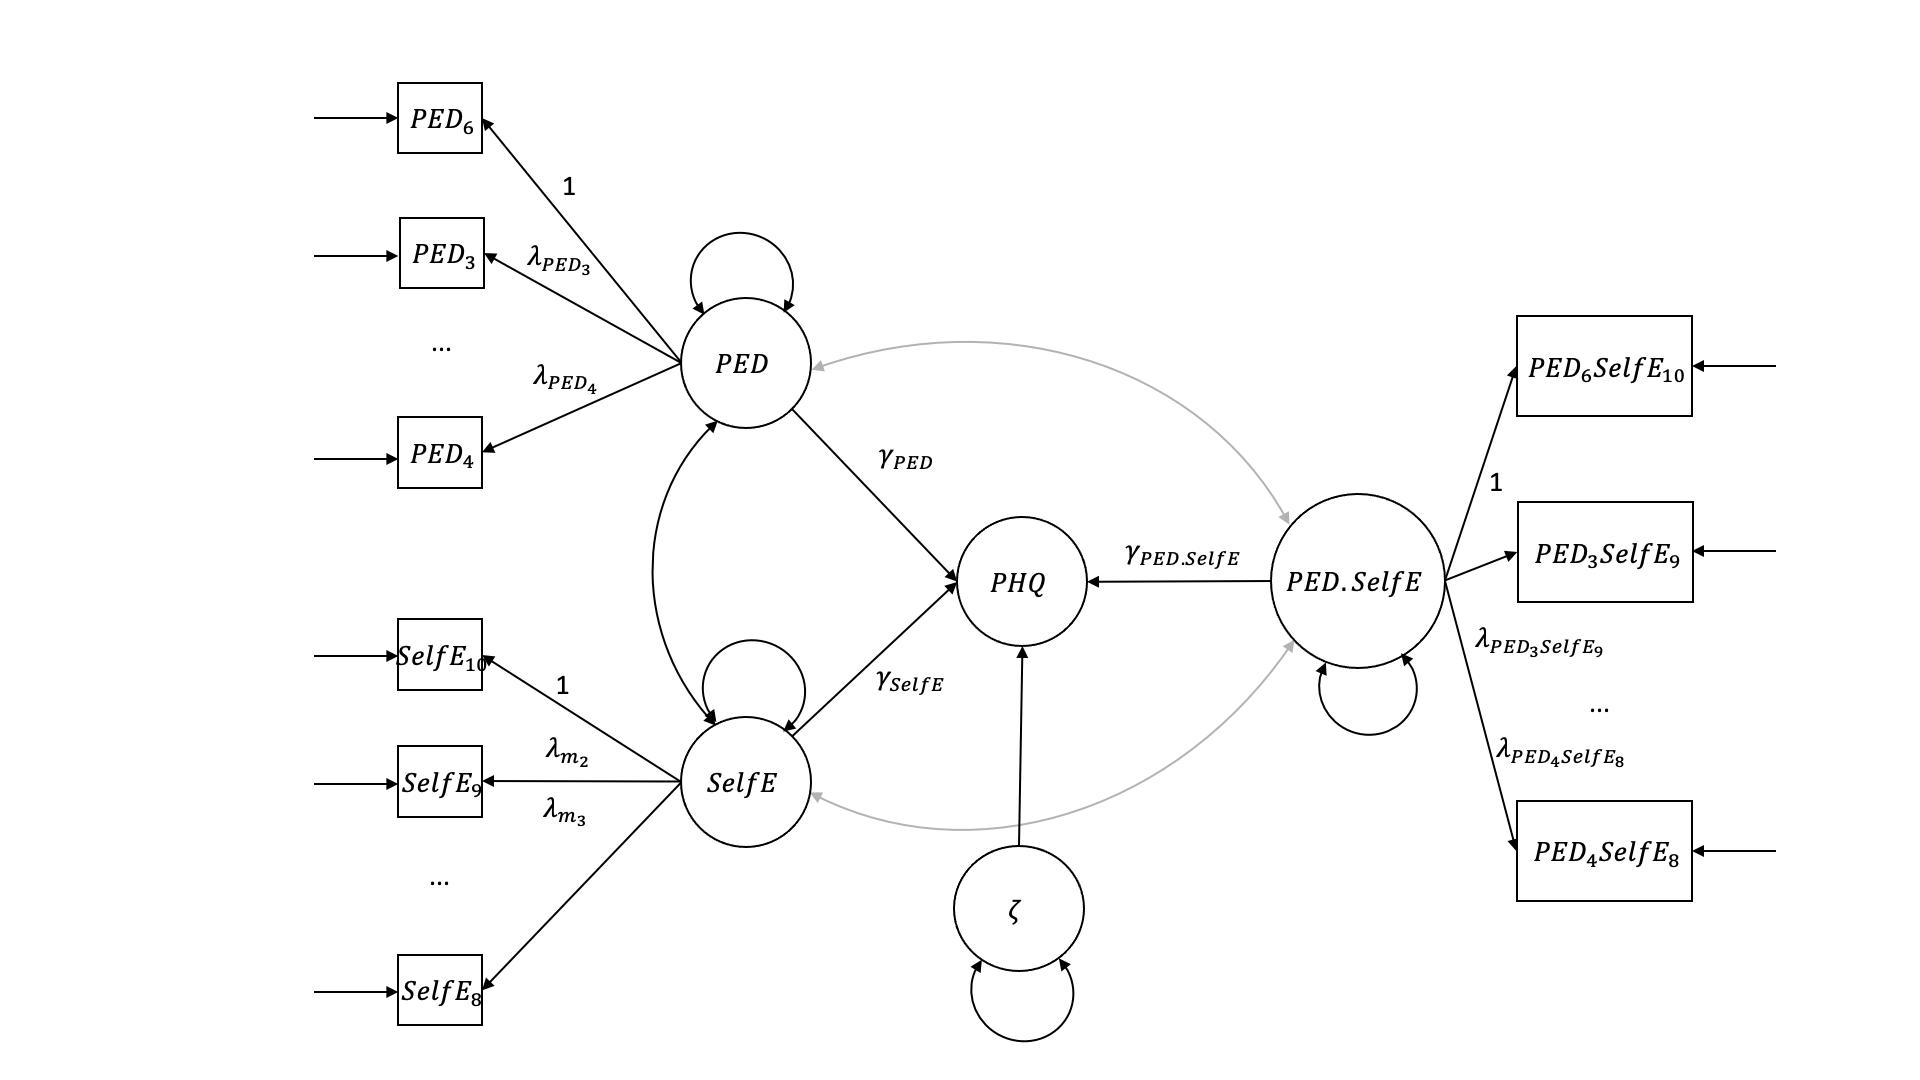
\includegraphics[width=1\linewidth]{Introduction/Plots/Slide1} 

}

\caption{Hypothesized Model of Matched-Pair UPI. PED, SelfE, and PHQ represent the latent variables of perceived everyday discrimination, self-esteem, and depression, which are indicated by their corresponding first-order indicators. The latent interaction term, PED.SelfE, is indicated by formed PIs. $\zeta$ is the disturbance of PHQ. The error terms of indicators were not shown due to limited space. PED, SelfE, and PED.SelfE are allowed to correlate with each other.}\label{fig:figure-1}
\end{figure}

\begin{figure}

{\centering 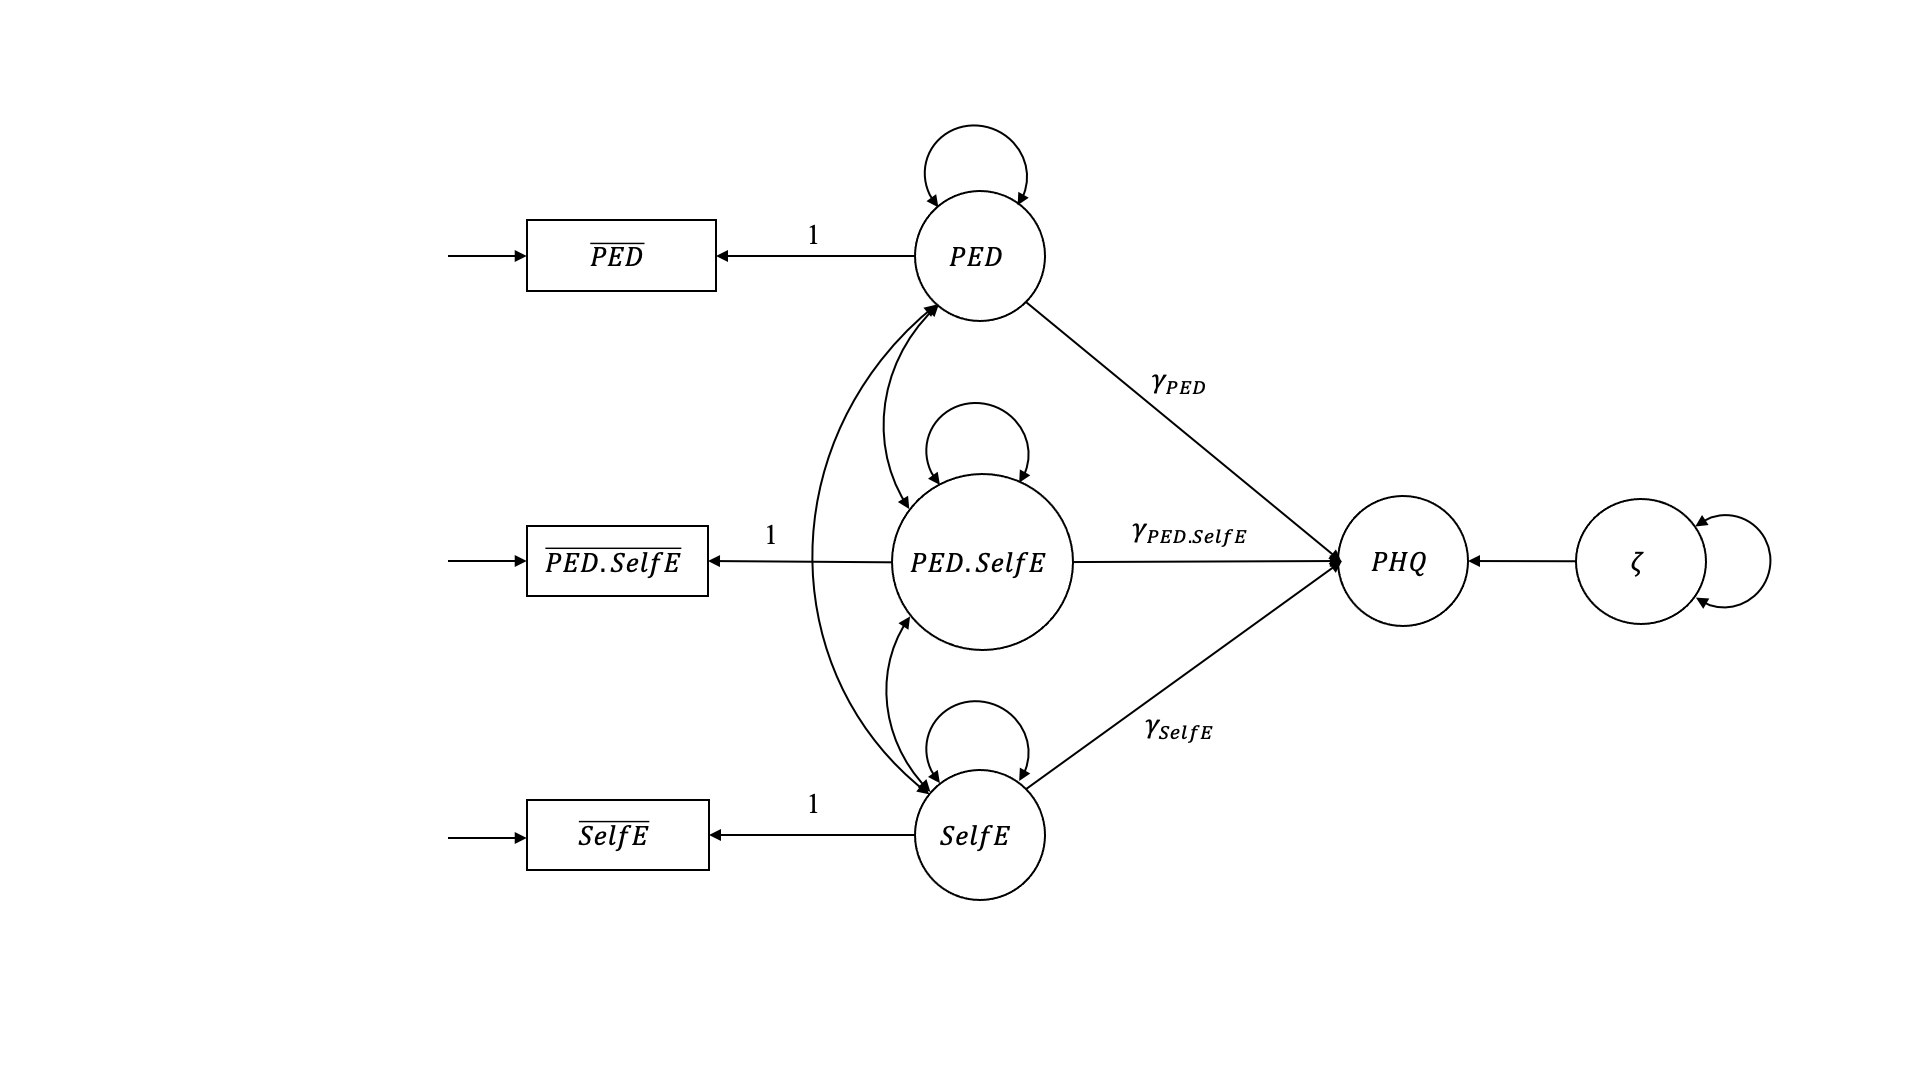
\includegraphics[width=1\linewidth]{Introduction/Plots/Slide2} 

}

\caption{Hypothesized Model of RAPI. PED, SelfE, and PHQ represent the latent variables of perceived everyday discrimination, self-esteem, and depression, which are indicated by corresponding single indicators using mean scores. The latent interaction term is indicated by the product of SIs of PED and SelfE. $\zeta$ is the disturbance of PHQ. The error terms of SIs were not shown due to limited space. PED, SelfE, and PED.SelfE are allowed to correlate with each other.}\label{fig:figure-2}
\end{figure}

\begin{figure}

{\centering 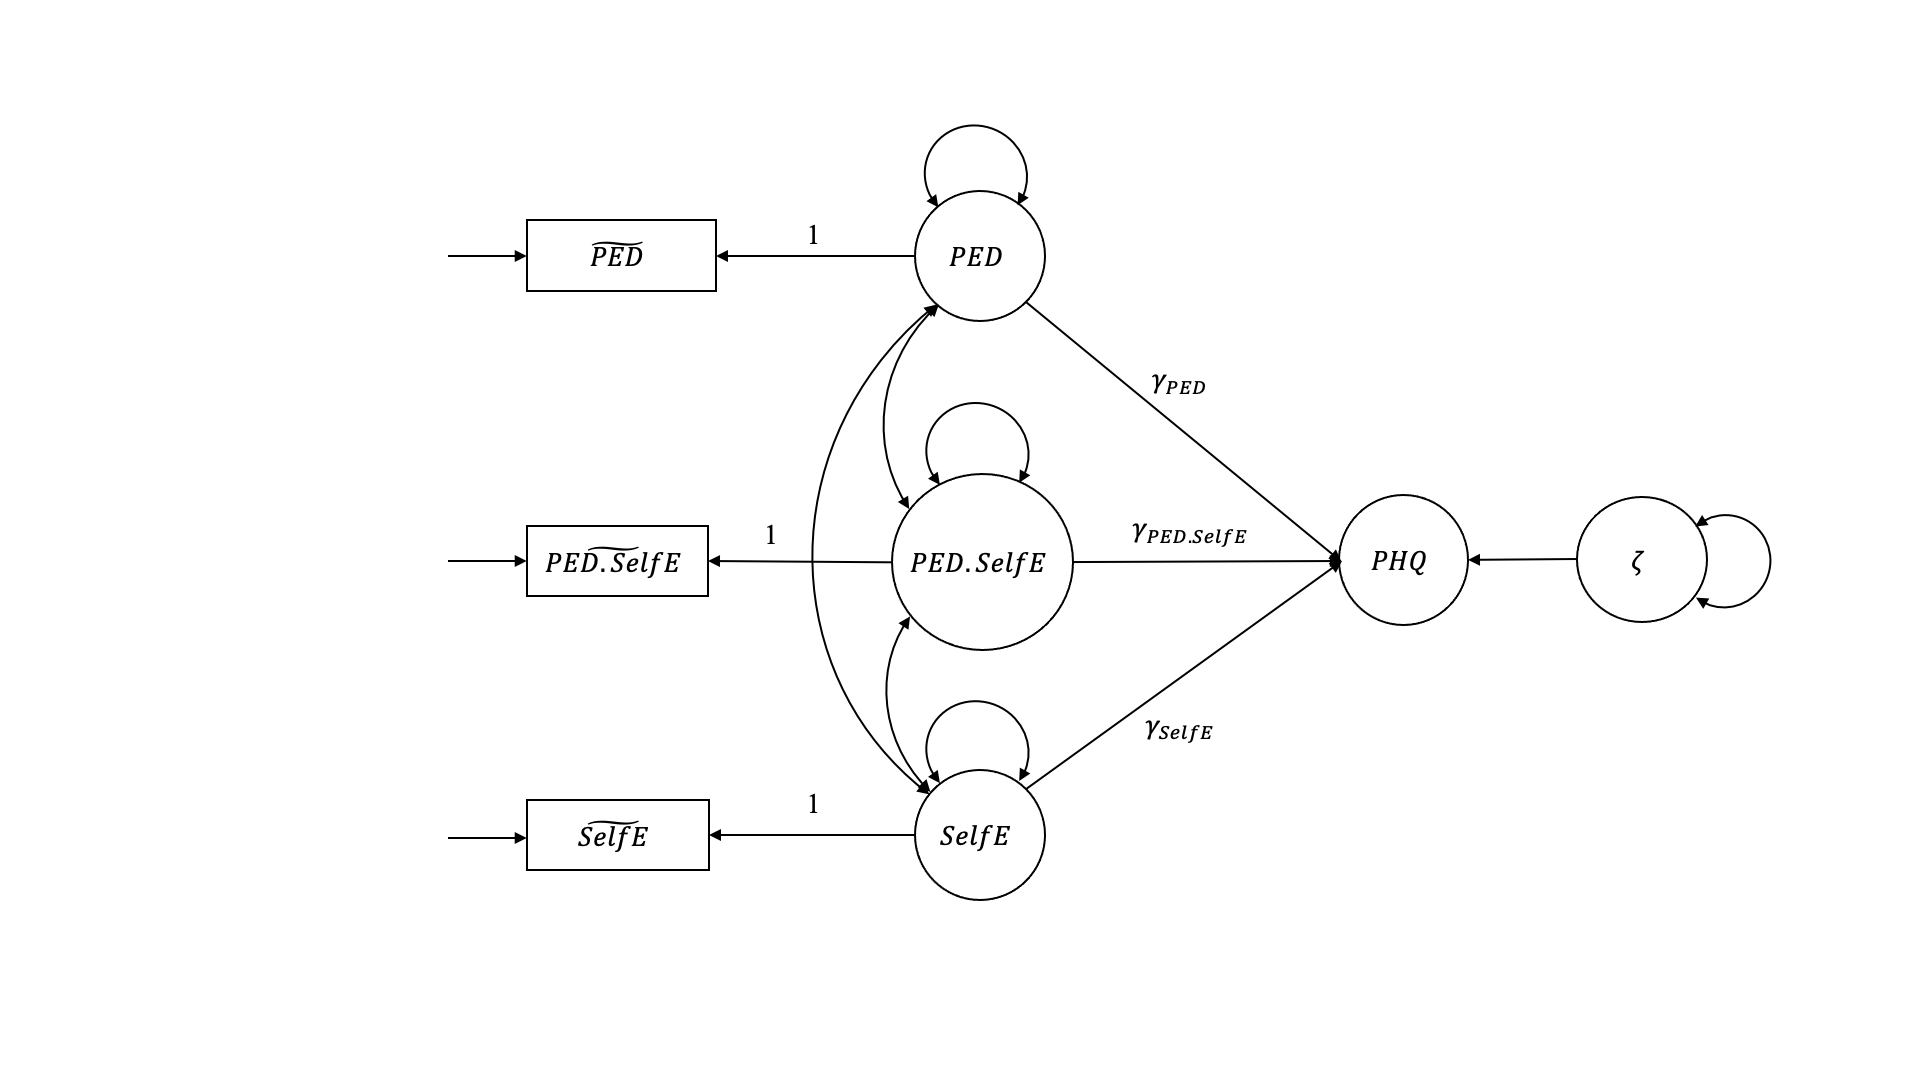
\includegraphics[width=1\linewidth]{Introduction/Plots/Slide3} 

}

\caption{Hypothesized Model of 2S-PA-Int. PED, SelfE, and PHQ represent the latent variables of perceived everyday discrimination, self-esteem, and depression, which are indicated by corresponding single indicators using factor scores. The latent interaction term is indicated by the product of SIs of PED and SelfE. $\zeta$ is the disturbance of PHQ. The error terms of SIs were not shown due to limited space. PED, SelfE, and PED.SelfE are allowed to correlate with each other.}\label{fig:figure-3}
\end{figure}

\newpage

\hypertarget{references}{%
\section{References}\label{references}}

\hypertarget{refs}{}
\begin{CSLReferences}{1}{0}
\leavevmode\vadjust pre{\hypertarget{ref-arnettEmergingAdulthoodTheory2000}{}}%
Arnett, J. J. (2000). Emerging adulthood: {A} theory of development from the late teens through the twenties. \emph{American Psychologist}, \emph{55}, 469--480. \url{https://doi.org/10.1037/0003-066X.55.5.469}

\leavevmode\vadjust pre{\hypertarget{ref-atkinsonStatisticalMethodsAssessing1998}{}}%
Atkinson, G., \& Nevill, A. M. (1998). Statistical methods for assessing measurement error (reliability) in variables relevant to sports medicine. \emph{Sports Med}, \emph{26}(4), 217--238. \url{https://doi.org/10.2165/00007256-199826040-00002}

\leavevmode\vadjust pre{\hypertarget{ref-baronModeratormediatorVariableDistinction1986}{}}%
Baron, R. M., \& Kenny, D. A. (1986). The moderator-mediator variable distinction in social psychological research: Conceptual, strategic, and statistical considerations. \emph{J Pers Soc Psychol}, \emph{51}(6), 1173--1182. \url{https://doi.org/10.1037//0022-3514.51.6.1173}

\leavevmode\vadjust pre{\hypertarget{ref-beckInventoryMeasuringClinical1988}{}}%
Beck, A. T., Epstein, N., Brown, G., \& Steer, R. A. (1988). An inventory for measuring clinical anxiety: {Psychometric} properties. \emph{Journal of Consulting and Clinical Psychology}, \emph{56}(6), 893--897. \url{https://doi.org/10.1037/0022-006X.56.6.893}

\leavevmode\vadjust pre{\hypertarget{ref-bollenStructuralEquationsLatent1989e}{}}%
Bollen, K. A. (1989). \emph{Structural equations with latent variables} (pp. xiv, 514). John Wiley \& Sons. \url{https://doi.org/10.1002/9781118619179}

\leavevmode\vadjust pre{\hypertarget{ref-browneAlternativeWaysAssessing1992}{}}%
Browne, M. W., \& Cudeck, R. (1992). Alternative ways of assessing model fit. \emph{Sociological Methods \& Research}, \emph{21}(2), 230--258. \url{https://doi.org/10.1177/0049124192021002005}

\leavevmode\vadjust pre{\hypertarget{ref-burgessEffectsPerceivedDiscrimination2007}{}}%
Burgess, D., Lee, R., Tran, A., \& van Ryn, M. (2007). Effects of perceived discrimination on mental health and mental health services utilization among gay, lesbian, bisexual and transgender persons. \emph{Journal of LGBT Health Research}, \emph{3}(4), 1--14. \url{https://doi.org/10.1080/15574090802226626}

\leavevmode\vadjust pre{\hypertarget{ref-busemeyerAnalysisMultiplicativeCombination1983}{}}%
Busemeyer, J. R., \& Jones, L. E. (1983). Analysis of multiplicative combination rules when the causal variables are measured with error. \emph{Psychological Bulletin}, \emph{93}(3), 549--562. \url{https://doi.org/10.1037/0033-2909.93.3.549}

\leavevmode\vadjust pre{\hypertarget{ref-chenRelationshipBiculturalIdentity2022}{}}%
Chen, W., Lin, Y., Yu, X., Zheng, W., Wu, S., Huang, M., Chen, W., \& Zhou, S. (2022). The {Relationship} between {Bicultural Identity Integration}, {Self-Esteem}, {Academic Resilience}, {Interaction Anxiousness}, and {School Belonging} among {University Students} with {Vocational Qualifications}. \emph{International Journal of Environmental Research and Public Health}, \emph{19}(6), 3632. \url{https://doi.org/10.3390/ijerph19063632}

\leavevmode\vadjust pre{\hypertarget{ref-chenSocioeconomicStatusLife2016}{}}%
Chen, W., Niu, G.-F., Zhang, D.-J., Fan, C.-Y., Tian, Y., \& Zhou, Z.-K. (2016). Socioeconomic status and life satisfaction in {Chinese} adolescents: {Analysis} of self-esteem as a mediator and optimism as a moderator. \emph{Personality and Individual Differences}, \emph{95}, 105--109. \url{https://doi.org/10.1016/j.paid.2016.01.036}

\leavevmode\vadjust pre{\hypertarget{ref-cronbachCoefficientAlphaInternal1951}{}}%
Cronbach, L. J. (1951). Coefficient alpha and the internal structure of tests. \emph{Psychometrika}, \emph{16}(3), 297--334. \url{https://doi.org/10.1007/BF02310555}

\leavevmode\vadjust pre{\hypertarget{ref-drRaceHealthBasic1997}{}}%
Dr, W. (1997). Race and health: {Basic} questions, emerging directions. \emph{Annals of Epidemiology}, \emph{7}(5). \url{https://doi.org/10.1016/s1047-2797(97)00051-3}

\leavevmode\vadjust pre{\hypertarget{ref-espinosaDiscriminationSelfEsteemMental2021a}{}}%
Espinosa, A. (2021). Discrimination, {Self-Esteem}, and {Mental Health Across Ethnic Groups} of {Second-Generation Immigrant Adolescents}. \emph{J. Racial and Ethnic Health Disparities}, \emph{8}(6), 1539--1550. \url{https://doi.org/10.1007/s40615-020-00917-1}

\leavevmode\vadjust pre{\hypertarget{ref-estabrookComparisonFactorScore2013a}{}}%
Estabrook, R., \& Neale, M. (2013). A comparison of factor score estimation methods in the presence of missing data: {Reliability} and an application to nicotine dependence. \emph{Multivariate Behavioral Research}, \emph{48}(1). \url{https://doi.org/10.1080/00273171.2012.730072}

\leavevmode\vadjust pre{\hypertarget{ref-fairchildEvaluatingMediationModeration2010}{}}%
Fairchild, A. J., \& McQuillin, S. D. (2010). Evaluating mediation and moderation effects in school psychology: {A} presentation of methods and review of current practice. \emph{Journal of School Psychology}, \emph{48}(1), 53--84. \url{https://doi.org/10.1016/j.jsp.2009.09.001}

\leavevmode\vadjust pre{\hypertarget{ref-fritzCombinedEffectsMeasurement2016}{}}%
Fritz, M. S., Kenny, D. A., \& MacKinnon, D. P. (2016). The combined effects of measurement error and omitting confounders in the single-mediator model. \emph{Multivariate Behavioral Research}, \emph{51}(5), 681--697. \url{https://doi.org/10.1080/00273171.2016.1224154}

\leavevmode\vadjust pre{\hypertarget{ref-hancockReliabilityAradoxAssessing2011}{}}%
Hancock, G. R., \& Mueller, R. O. (2011). The reliability aradox in assessing structural relations within covariance structure models. \emph{Educational and Psychological Measurement}, \emph{71}(2), 306--324. \url{https://doi.org/10.1177/0013164410384856}

\leavevmode\vadjust pre{\hypertarget{ref-harterDevelopmentSelfrepresentationsChildhood2003}{}}%
Harter, S. (2003). The development of self-representations during childhood and adolescence. In \emph{Handbook of self and identity} (pp. 610--642). The Guilford Press.

\leavevmode\vadjust pre{\hypertarget{ref-hayesIntroductionMediationModeration2013}{}}%
Hayes, A. F. (2013). \emph{Introduction to mediation, moderation, and conditional process analysis: {A} regression-based approach} (pp. xvii, 507). Guilford Press.

\leavevmode\vadjust pre{\hypertarget{ref-hayesRegressionbasedStatisticalMediation2017}{}}%
Hayes, A. F., \& Rockwood, N. J. (2017). Regression-based statistical mediation and moderation analysis in clinical research: {Observations}, recommendations, and implementation. \emph{Behav Res Ther}, \emph{98}, 39--57. \url{https://doi.org/10.1016/j.brat.2016.11.001}

\leavevmode\vadjust pre{\hypertarget{ref-hoyleStructuralEquationModeling1995}{}}%
Hoyle, R. H. (1995). The structural equation modeling approach: {Basic} concepts and fundamental issues. In \emph{Structural equation modeling: {Concepts}, issues, and applications} (pp. 1--15). Sage Publications, Inc.

\leavevmode\vadjust pre{\hypertarget{ref-hsiaoEvaluationTwoMethods2018b}{}}%
Hsiao, Y.-Y., Kwok, O.-M., \& Lai, M. H. C. (2018). Evaluation of two methods for modeling measurement errors when testing interaction effects with observed composite scores. \emph{Educ Psychol Meas}, \emph{78}(2), 181--202. \url{https://doi.org/10.1177/0013164416679877}

\leavevmode\vadjust pre{\hypertarget{ref-hsiaoModelingMeasurementErrors2021a}{}}%
Hsiao, Y.-Y., Kwok, O.-M., \& Lai, M. H. C. (2021). Modeling measurement errors of the exogenous composites from congeneric measures in interaction models. \emph{Struct Equ Modeling}, \emph{28}(2), 250--260. \url{https://doi.org/10.1080/10705511.2020.1782206}

\leavevmode\vadjust pre{\hypertarget{ref-huCutoffCriteriaFit1999}{}}%
Hu, L., \& Bentler, P. M. (1999). Cutoff criteria for fit indexes in covariance structure analysis: {Conventional} criteria versus new alternatives. \emph{Structural Equation Modeling}, \emph{6}(1), 1--55. \url{https://doi.org/10.1080/10705519909540118}

\leavevmode\vadjust pre{\hypertarget{ref-InstituteSocialResearch2024a}{}}%
\emph{Institute for social research}. (2024). https://isr-umich-edu.libproxy1.usc.edu/.

\leavevmode\vadjust pre{\hypertarget{ref-jaccardMeasurementErrorAnalysis1995}{}}%
Jaccard, J., \& Wan, C. K. (1995). Measurement error in the analysis of interaction effects between continuous predictors using multiple regression: {Multiple} indicator and structural equation approaches. \emph{Psychological Bulletin}, \emph{117}(2), 348--357. \url{https://doi.org/10.1037/0033-2909.117.2.348}

\leavevmode\vadjust pre{\hypertarget{ref-joreskogLISRELStructuralEquation1993}{}}%
Jöreskog, K. G., \& Sörbom, D. (1993). \emph{{LISREL} 8: {Structural} equation modeling with the {SIMPLIS} command language} (pp. xvi, 202). Lawrence Erlbaum Associates, Inc.

\leavevmode\vadjust pre{\hypertarget{ref-jorgensen2022}{}}%
Jorgensen, T. D., Pornprasertmanit, S., Schoemann, A. M., \& Rosseel, Y. (2022). \emph{\texttt{semTools}: {U}seful tools for structural equation modeling}. \url{https://CRAN.R-project.org/package=semTools}

\leavevmode\vadjust pre{\hypertarget{ref-kennyEstimatingNonlinearInteractive1984b}{}}%
Kenny, D. A., \& Judd, C. M. (1984). Estimating the nonlinear and interactive effects of latent variables. \emph{Psychological Bulletin}, \emph{96}(1), 201--210. \url{https://doi.org/10.1037/0033-2909.96.1.201}

\leavevmode\vadjust pre{\hypertarget{ref-kiraAreNegativeMental2015}{}}%
Kira, I. A., Omidy, A. Z., Fawzi, M., Rice, K. G., Fawzi, M., Lewandowski, L., \& Bujold-Bugeaud, M. (2015). Are the negative mental health effects of gender discrimination ({GD}) salient across cultures? {Does} self-esteem mediate these effects: {GD} as a continuous traumatic stress and the pathways to its negative dynamics? \emph{Psychology}, \emph{6}(1), 93--116. \url{https://doi.org/10.4236/psych.2015.61009}

\leavevmode\vadjust pre{\hypertarget{ref-kleinMaximumLikelihoodEstimation2000}{}}%
Klein, A., \& Moosbrugger, H. (2000). Maximum likelihood estimation of latent interaction effects with the {LMS} method. \emph{Psychometrika}, \emph{65}(4), 457--474. \url{https://doi.org/10.1007/BF02296338}

\leavevmode\vadjust pre{\hypertarget{ref-klinePrinciplesPracticeStructural2016a}{}}%
Kline, R. B. (2016). \emph{Principles and practice of structural equation modeling, 4th ed} (pp. xvii, 534). Guilford Press.

\leavevmode\vadjust pre{\hypertarget{ref-klodnickMeetingDevelopmentalNeeds2021}{}}%
Klodnick, V. V., Malina, C., Fagan, M. A., Johnson, R. P., Brenits, A., Zeidner, E., \& Viruet, J. (2021). Meeting the developmental needs of young adults diagnosed with serious mental health challenges: The emerge model. \emph{J Behav Health Serv Res}, \emph{48}(1), 77--92. \url{https://doi.org/10.1007/s11414-020-09699-0}

\leavevmode\vadjust pre{\hypertarget{ref-kroenkeAnxietyDisordersPrimary2007}{}}%
Kroenke, K., Spitzer, R. L., Williams, J. B. W., Monahan, P. O., \& Löwe, B. (2007). Anxiety disorders in primary care: {Prevalence}, impairment, comorbidity, and detection. \emph{Ann Intern Med}, \emph{146}(5), 317--325. \url{https://doi.org/10.7326/0003-4819-146-5-200703060-00004}

\leavevmode\vadjust pre{\hypertarget{ref-laiTwostagePathAnalysis2022a}{}}%
Lai, M. H. C., \& Hsiao, Y.-Y. (2022). Two-stage path analysis with definition variables: {An} alternative framework to account for measurement error. \emph{Psychological Methods}, \emph{27}(4), 568--588. \url{https://doi.org/10.1037/met0000410}

\leavevmode\vadjust pre{\hypertarget{ref-laiCorrectingUnreliabilityPartial2023}{}}%
Lai, M. H. C., Tse, W. W.-Y., Zhang, G., Li, Y., \& Hsiao, Y.-Y. (2023). Correcting for unreliability and partial invariance: {A} two-stage path analysis approach. \emph{Structural Equation Modeling: A Multidisciplinary Journal}, \emph{30}(2), 258--271. \url{https://doi.org/10.1080/10705511.2022.2125397}

\leavevmode\vadjust pre{\hypertarget{ref-linStructuralEquationModels2010b}{}}%
Lin, G.-C., Wen, Z., Marsh, H. W., \& Lin, H.-S. (2010). Structural equation models of latent interactions: {Clarification} of orthogonalizing and double-mean-centering strategies. \emph{Structural Equation Modeling: A Multidisciplinary Journal}, \emph{17}(3), 374--391. \url{https://doi.org/10.1080/10705511.2010.488999}

\leavevmode\vadjust pre{\hypertarget{ref-lodderModelingInteractionsLatent2019}{}}%
Lodder, P., Denollet, J., Emons, W. H. M., Nefs, G., Pouwer, F., Speight, J., \& Wicherts, J. M. (2019). Modeling interactions between latent variables in research on {Type D} personality: {A} monte carlo simulation and clinical study of depression and anxiety. \emph{Multivariate Behav Res}, \emph{54}(5), 637--665. \url{https://doi.org/10.1080/00273171.2018.1562863}

\leavevmode\vadjust pre{\hypertarget{ref-marshStructuralEquationModels2004b}{}}%
Marsh, H. W., Wen, Z., \& Hau, K.-T. (2004). Structural equation models of latent interactions: Evaluation of alternative estimation strategies and indicator construction. \emph{Psychol Methods}, \emph{9}(3), 275--300. \url{https://doi.org/10.1037/1082-989X.9.3.275}

\leavevmode\vadjust pre{\hypertarget{ref-marshStructuralEquationModels2012}{}}%
Marsh, H. W., Wen, Z., Nagengast, B., \& Hau, K.-T. (2012). Structural equation models of latent interaction. In \emph{Handbook of structural equation modeling} (pp. 436--458). The Guilford Press.

\leavevmode\vadjust pre{\hypertarget{ref-martinez-hernaezSocialSupportGender2016}{}}%
Martínez-Hernáez, A., Carceller-Maicas, N., DiGiacomo, S. M., \& Ariste, S. (2016). Social support and gender differences in coping with depression among emerging adults: A mixed-methods study. \emph{Child and Adolescent Psychiatry and Mental Health}, \emph{10}(1), 2. \url{https://doi.org/10.1186/s13034-015-0088-x}

\leavevmode\vadjust pre{\hypertarget{ref-maslowskyEstimatingInterpretingLatent2015b}{}}%
Maslowsky, J., Jager, J., \& Hemken, D. (2015). Estimating and interpreting latent variable interactions: {A} tutorial for applying the latent moderated structural equations method. \emph{International Journal of Behavioral Development}, \emph{39}(1), 87--96. \url{https://doi.org/10.1177/0165025414552301}

\leavevmode\vadjust pre{\hypertarget{ref-mcdonaldTheoreticalFoundationsPrincipal1970a}{}}%
McDonald, R. P. (1970). The theoretical foundations of principal factor analysis, canonical factor analysis, and alpha factor analysis. \emph{British Journal of Mathematical and Statistical Psychology}, \emph{23}(1), 1--21. \url{https://doi.org/10.1111/j.2044-8317.1970.tb00432.x}

\leavevmode\vadjust pre{\hypertarget{ref-nakagawaFarewellBonferroniProblems2004}{}}%
Nakagawa, S. (2004). A farewell to {Bonferroni}: {The} problems of low statistical power and publication bias. \emph{Behavioral Ecology}, \emph{15}(6), 1044--1045. \url{https://doi.org/10.1093/beheco/arh107}

\leavevmode\vadjust pre{\hypertarget{ref-ngDoesBystanderBehavior2022}{}}%
Ng, K., Niven, K., \& Notelaers, G. (2022). Does bystander behavior make a difference? {How} passive and active bystanders in the group moderate the effects of bullying exposure. \emph{Journal of Occupational Health Psychology}, \emph{27}(1), 119--135. \url{https://doi.org/10.1037/ocp0000296}

\leavevmode\vadjust pre{\hypertarget{ref-nunnallyPsychometricTheory1994a}{}}%
Nunnally, J. C., \& Bernstein, I. H. (1994). \emph{Psychometric theory} (3rd ed). McGraw-Hill.

\leavevmode\vadjust pre{\hypertarget{ref-PanelStudyIncome2019a}{}}%
\emph{Panel {Study} of {Income Dynamics} {[}{Transition} into {Adulthood Supplement}{]}, public use dataset}. (2019). the Survey Research Center, Institute for Social Research, University of Michigan, Ann Arbor, MI.

\leavevmode\vadjust pre{\hypertarget{ref-pascoePerceivedDiscriminationHealth2009a}{}}%
Pascoe, E. A., \& Richman, L. S. (2009). Perceived discrimination and health: {A} meta-analytic review. \emph{Psychol Bull}, \emph{135}(4), 531--554. \url{https://doi.org/10.1037/a0016059}

\leavevmode\vadjust pre{\hypertarget{ref-patrickEffectRacialDiscrimination2019}{}}%
Patrick, A. A. (2019). The effect of racial discrimination on mental health of {African American} and {Hispanic American} adolescents. In \emph{Dissertation Abstracts International Section A: Humanities and Social Sciences} (PhD Thesis 7-A(E); Vol. 80). ProQuest Information \& Learning (US).

\leavevmode\vadjust pre{\hypertarget{ref-pingEQSLISRELExamples1998}{}}%
Ping, R. A. (1998). {EQS} and {LISREL} examples using survey data. In \emph{Interaction and {Nonlinear Effects} in {Structural Equation Modeling}}. Routledge.

\leavevmode\vadjust pre{\hypertarget{ref-raykovEstimationCompositeReliability1997}{}}%
Raykov, T. (1997). Estimation of composite reliability for congeneric measures. \emph{Applied Psychological Measurement}, \emph{21}(2), 173--184. \url{https://doi.org/10.1177/01466216970212006}

\leavevmode\vadjust pre{\hypertarget{ref-rosenbergRosenbergSelfEsteemScale1965}{}}%
Rosenberg, M. (1965). \emph{Rosenberg {Self-Esteem Scale}}. \url{https://doi.org/10.1037/t01038-000}

\leavevmode\vadjust pre{\hypertarget{ref-rosenbergSocietyAdolescentSelfimage2015}{}}%
Rosenberg, M. (2015). \emph{Society and the adolescent self-image}. Princeton University Press.

\leavevmode\vadjust pre{\hypertarget{ref-rosseelLavaanPackageStructural2012}{}}%
Rosseel, Y. (2012). Lavaan: {An R} package for structural equation modeling. \emph{Journal of Statistical Software}, \emph{48}, 1--36. \url{https://doi.org/10.18637/jss.v048.i02}

\leavevmode\vadjust pre{\hypertarget{ref-tenbergeGreatestLowerBound2004a}{}}%
Ten Berge, J. M. F., \& Sočan, G. (2004). The greatest lower bound to the reliability of a test and the hypothesis of unidimensionality. \emph{Psychometrika}, \emph{69}(4), 613--625. \url{https://doi.org/10.1007/BF02289858}

\leavevmode\vadjust pre{\hypertarget{ref-wagnerLongitudinalTransitionOutcomes2012}{}}%
Wagner, M., \& Newman, L. (2012). Longitudinal transition outcomes of youth with emotional disturbances. \emph{Psychiatr Rehabil J}, \emph{35}(3), 199--208. \url{https://doi.org/10.2975/35.3.2012.199.208}

\leavevmode\vadjust pre{\hypertarget{ref-wallGeneralizedAppendedProduct2001}{}}%
Wall, M. M., \& Amemiya, Y. (2001). Generalized appended product indicator procedure for nonlinear structural equation analysis. \emph{Journal of Educational and Behavioral Statistics}, \emph{26}(1), 1--30. \url{https://doi.org/10.3102/10769986026001001}

\leavevmode\vadjust pre{\hypertarget{ref-weinbergFoundationsSportExercise1995}{}}%
Weinberg, R. S., \& Gould, D. (1995). \emph{Foundations of sport and exercise psychology} (pp. xiv, 529). Human Kinetics Publishers.

\leavevmode\vadjust pre{\hypertarget{ref-williamsRacialEthnicDiscrimination2003}{}}%
Williams, D. R., Neighbors, H. W., \& Jackson, J. S. (2003). Racial/ethnic discrimination and health: {Findings} from community studies. \emph{Am J Public Health}, \emph{93}(2), 200--208. \url{https://doi.org/10.2105/AJPH.93.2.200}

\leavevmode\vadjust pre{\hypertarget{ref-wuAppropriateStandardizedEstimates2011}{}}%
Wu, Y., Wen, Z. L., Hau, K.-T., \& Marsh, H. (2011). Appropriate standardized estimates of latent interaction models without the mean structure. \emph{Acta Psychologica Sinica}, \emph{43}, 1219--1228.

\leavevmode\vadjust pre{\hypertarget{ref-wuComparisonStrategiesForming2013a}{}}%
Wu, Y., Wen, Z., Marsh, H. W., \& Hau, K.-T. (2013). A comparison of strategies for forming product indicators for unequal numbers of items in structural equation models of latent interactions. \emph{Structural Equation Modeling: A Multidisciplinary Journal}, \emph{20}(4), 551--567. \url{https://doi.org/10.1080/10705511.2013.824772}

\leavevmode\vadjust pre{\hypertarget{ref-yezerinacMeasurementErrorMorphometric1992}{}}%
Yezerinac, S. M., Lougheed, S. C., \& Handford, P. (1992). Measurement error and morphometric studies: {Statistical} power and observer experience. \emph{Systematic Biology}, \emph{41}(4), 471--482. \url{https://doi.org/10.2307/2992588}

\end{CSLReferences}


\end{document}
